As a first step in the evaluation of our evolutionary program synthesis method, we consider two PDE-based model problems, Poisson's equation and a linear elastic boundary value problem, which can already be solved efficiently by applying common multigrid cycles iteratively.
Here, our goal is, first of all, to demonstrate that our approach is able to reliably find functioning multigrid cycles in a number of randomized independent experiments.
Furthermore, since the known multigrid cycles already provide a strong baseline for these problems, we can investigate whether the methods designed with our approach are able to achieve a similar degree of efficiency.
In addition, by considering both two- and three-dimensional problems as well as a system of PDEs, we can demonstrate that our implementation is able to handle PDEs of different types.
\section{Automating the Design of Multigrid Cycles for Common PDEs}
\label{sec:experiments-part1}
As it has been mentioned above, the goal of this section is to evaluate the effectiveness of our evolutionary program synthesis method for the automated design of multigrid cycles that are able to quickly reduce the error of a given discretized PDE.
Therefore, the problem instances considered in this section are chosen in a way that facilitates their efficient solution by multigrid.
This is reflected in the fact that common multigrid cycles, as described in Section~\ref{sec:multigrid-cycles}, are able to quickly converge to the correct solution of each of the resulting systems of linear equations.
We begin this section by introducing the considered problem instances and their mathematical formulation.
At this point, we want to emphasize that all results presented in this section have been originally published as part of the paper~\cite{schmitt2021evostencils}.
However, this thesis complements this work with an additional analysis of the multigrid solvers obtained by our evolutionary search method.
\subsection{Problem Formulation}
\subsubsection{Poisson's Equation}
\label{sec:poisson-equation}
Poisson's equation is an elliptic PDE that occurs in the study of many physical phenomena~\cite{folland2020introduction} and is defined as
\begin{equation}
	\begin{split}
		-\nabla^{2} u & = f \quad \text{in} \; \Omega \\
		u & = g \quad \text{on} \; \partial \Omega.
	\end{split}
	\label{eq:poisson}
\end{equation}
In our experimental evaluation, we consider two different instances of Poisson's equation with Dirichlet boundary conditions, which are summarized in Table~\ref{table:poisson-problems}.
\begin{table}
	\begin{tabular}{r l l}
		\toprule
		Problem & 2D Poisson & 3D Poisson \\
		\midrule
		$\Omega = $ & $ (0, 1)^2$ & $(0, 1)^3$ \\
		\midrule
		$f(\bm{x}) = $ & $\pi^2 \cos(\pi x) - 4 \pi^2 \sin(2 \pi y)$ & $x^2 - 0.5 y^2 - 0.5 z^2$ \\
		\midrule
		$g(\bm{x}) = $ & $\cos(\pi x) - \sin(\pi y)$ & $0$ \\
		\bottomrule
	\end{tabular}
	\caption{Poisson problem instances.}
	\label{table:poisson-problems}
\end{table}
Note that in Section~\ref{sec:execution-time-analysis}, we have employed the same two-dimensional instance of Poisson's equation to estimate the relative cost of each operation within our evolutionary search method.
We discretize the Laplace operator $\nabla^{2}$ with finite differences on a uniform cartesian grid with step size $h = 1/2^{l_{max}}$, which yields the five-point stencil
\begin{equation*}
	\nabla^2_h = 
	\frac{1}{h^2} \begin{bmatrix}
		0 & 1 & 0\\
		1 & -4 & 1 \\
		0 & 1 & 0  
	\end{bmatrix},
\end{equation*}
in two dimensions, and the seven-point stencil
\begin{equation*}
\nabla^2_h = 
\frac{1}{h^2} \begin{bmatrix}
	\begin{bmatrix}
	0 & 0 & 0 \\
	0 & 1 & 0 \\
	0 & 0 & 0
	\end{bmatrix}
	&		
	\begin{bmatrix}
	0 & 1 & 0 \\
	1 & -6 & 1 \\
	0 & 1 & 0 
	\end{bmatrix} &
	\begin{bmatrix}
	0 & 0 & 0 \\
	0 & 1 & 0 \\
	0 & 0 & 0
\end{bmatrix}
\end{bmatrix}
\end{equation*} in three dimensions.
We choose a maximum level of $l_{max} = 11$ in 2D and $l_{max} = 7$ in 3D, which results in systems of linear equations consisting of $4\,190\,209$ and $2\,048\,383$ unknowns, respectively.

\subsubsection{Linear Elasticity}
Linear elasticity is a fundamental branch of solid mechanics with numerous applications in engineering and material science~\cite{holzapfel2001nonlinear}.
It is derived from the more general theory of nonlinear continuum mechanics by assuming a linear relationship between stress and strain during elastic deformation.
We consider a two-dimensional linear elastic boundary value problem given by the system of PDEs
\begin{equation}
	\begin{split}
		(\alpha + \beta) \cdot (\frac{\partial^2}{\partial x^2} u + \frac{\partial^2}{\partial x \partial y} v) + \alpha \nabla^2 u & = 0 \quad \text{in} \; \Omega \\
		(\alpha + \beta) \cdot (\frac{\partial^2}{\partial x \partial y} u + \frac{\partial^2}{\partial y^2} v) + \alpha \nabla^2 v & = 0 \quad \text{in} \; \Omega \\
		u = 0 \quad \text{and} \quad v & = g \quad \text{on} \; \partial \Omega 
		\label{eq:linear-elasticity}
	\end{split}
\end{equation}
where $\Omega = (0,1)^2$, $\alpha = 195$, $\beta = 130$ and
\begin{equation*}
	g(x,y) = 0.4 \, (1 - x) \, x y \, \sin(\pi x).
\end{equation*}
From a physical point of view, this system can be interpreted as a two-dimensional rectangular body that undergoes an elastic deformation into the y-direction, as it can be seen in Figure~\ref{fig:visualization-linear-elasticity}.
\begin{figure}
	\centering
	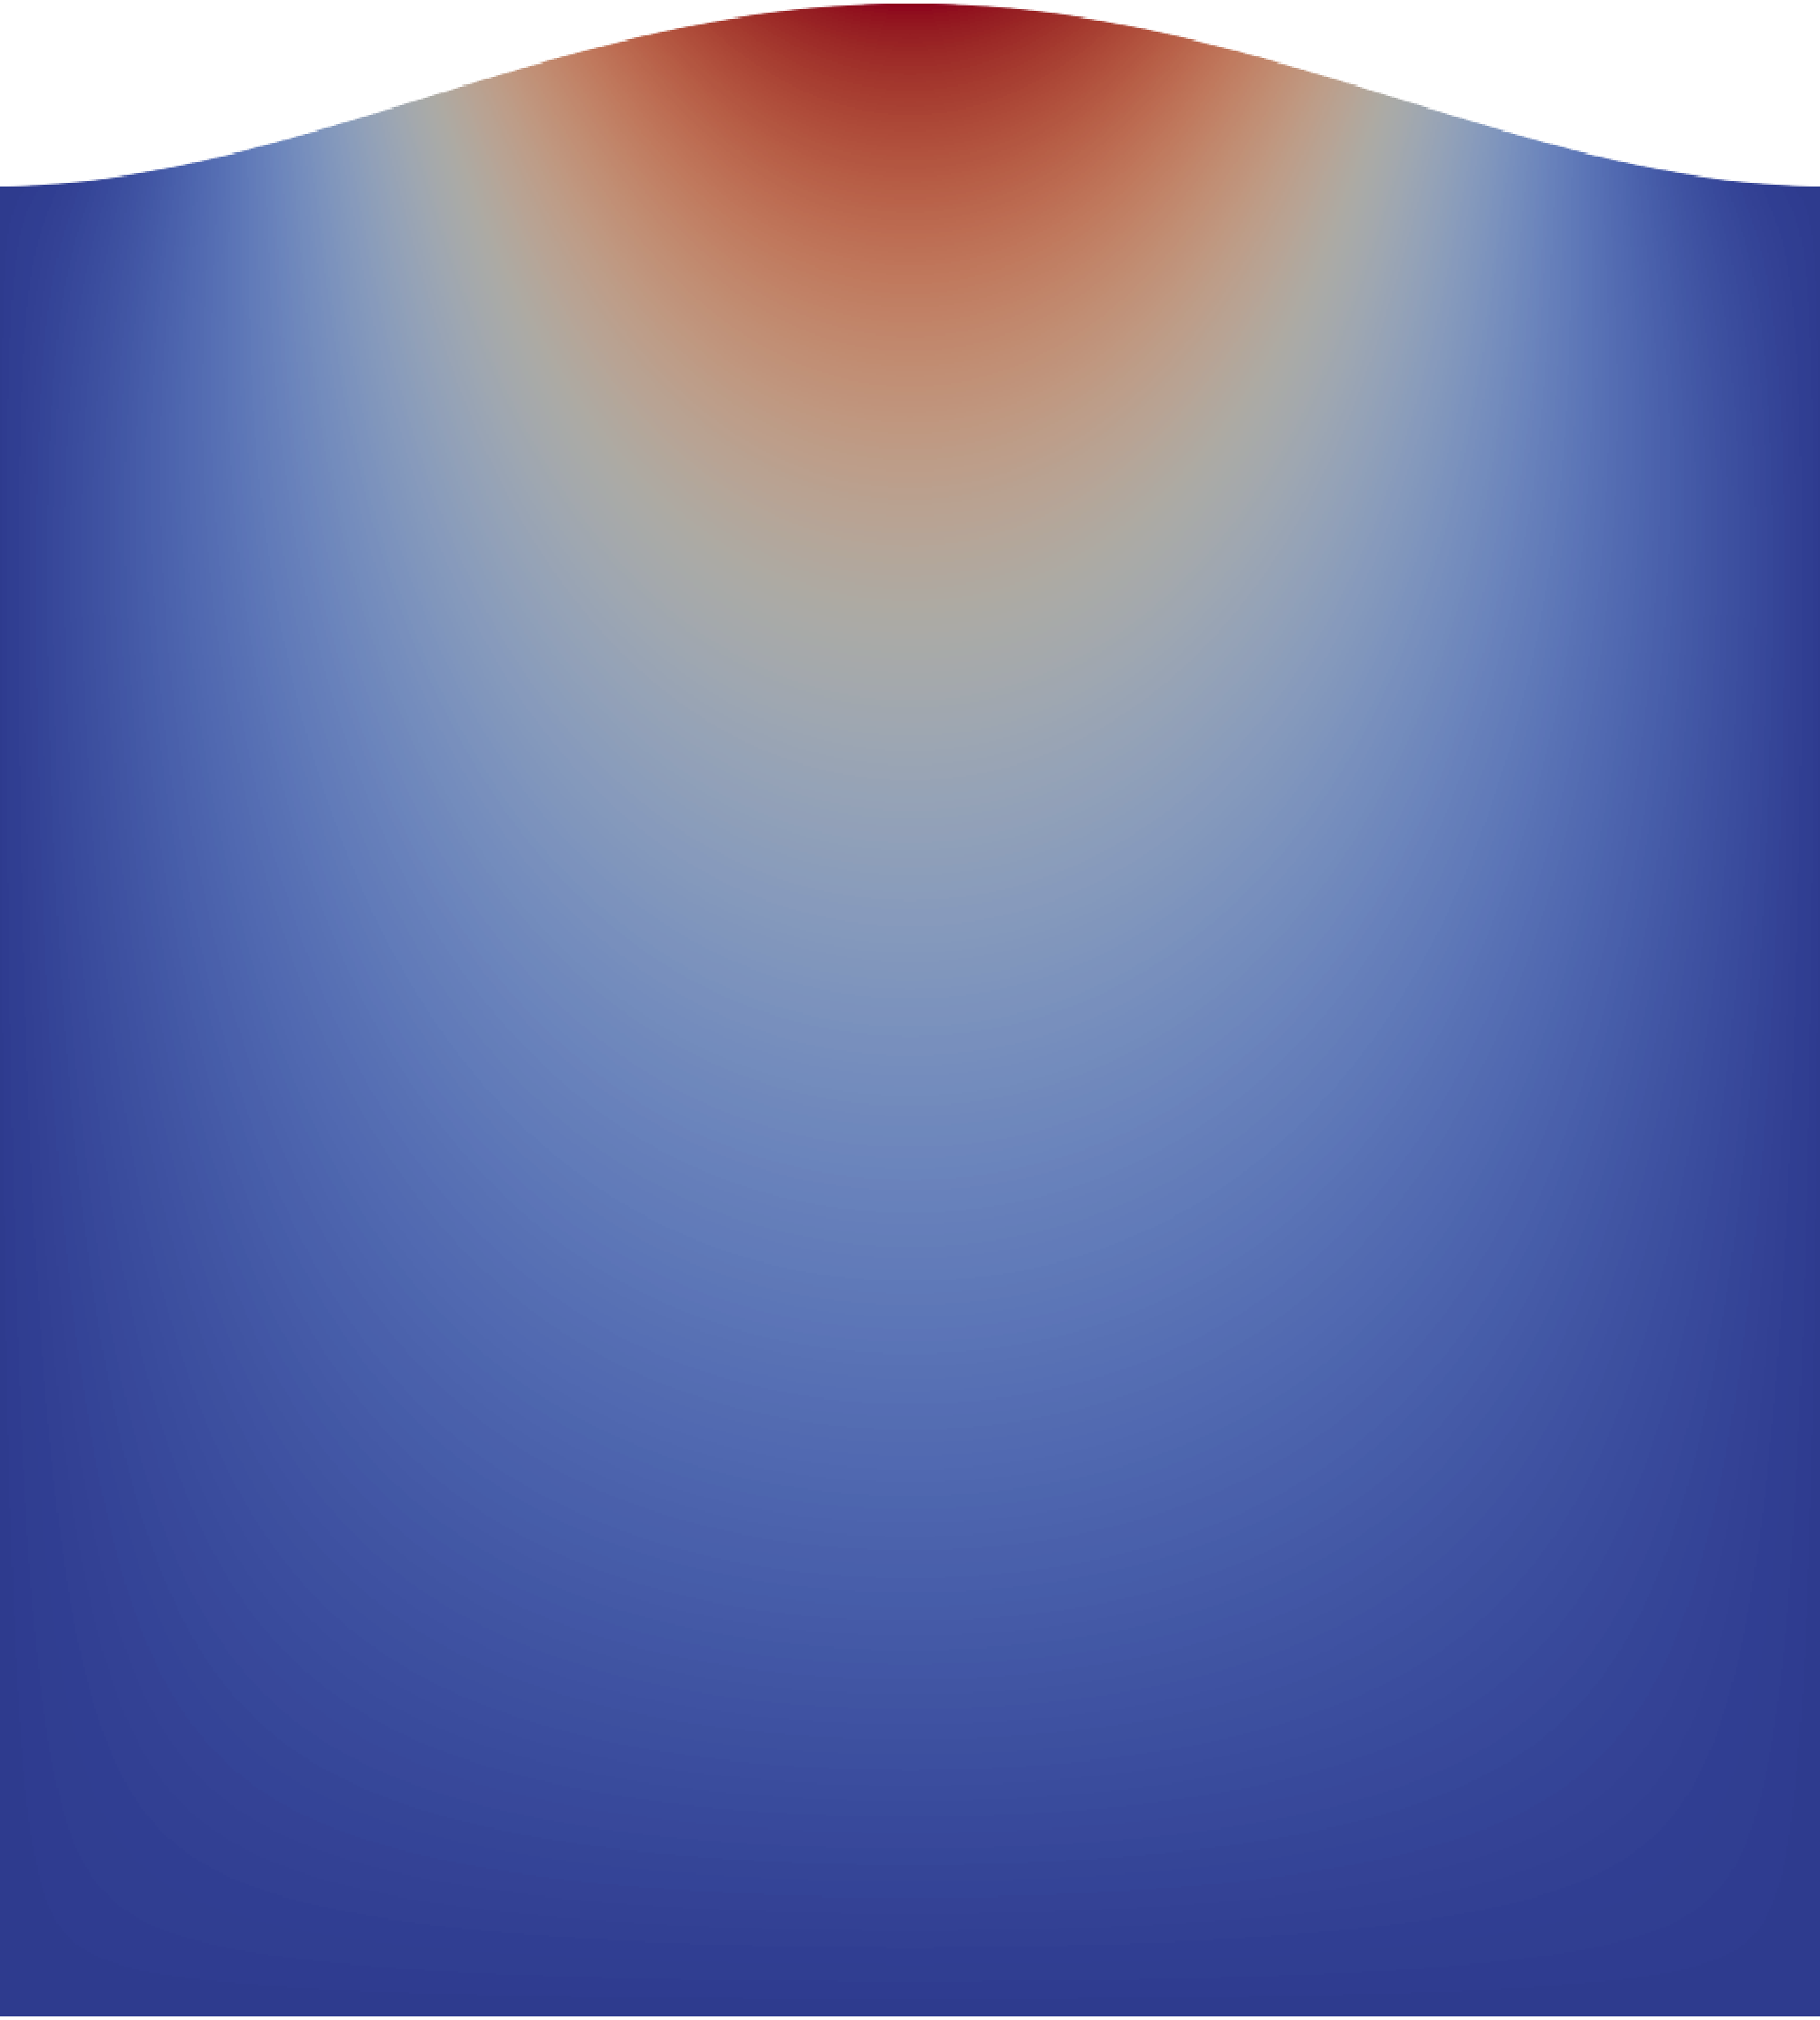
\includegraphics[width=0.5\textwidth]{figures/visualization-linear-elasticity1}
	\caption{Visualization of the considered linear elastic boundary value problem. A two-dimensional rectangular body undergoes an elastic deformation into the y-direction.}
	\label{fig:visualization-linear-elasticity}
\end{figure}
We discretize Equation \eqref{eq:linear-elasticity} with finite differences on a cartesian grid using a step size $h = 1/2^{l_{max}}$ with $l_{max} = 10$, which yields a system of linear equations $\bm{A} \bm{u} = \bm{f}$ with 
\begin{equation*}
	\bm{A} =
	\begin{pmatrix}
		(\alpha + \beta) \frac{\partial^2}{\partial x^2} + \alpha \nabla^2 & (\alpha + \beta) \frac{\partial^2}{\partial x \partial y} \\
		(\alpha + \beta) \frac{\partial^2}{\partial x \partial y} & (\alpha + \beta) \frac{\partial^2}{\partial y^2} +  \alpha \nabla^2
	\end{pmatrix},
\end{equation*}
\begin{equation*}
	\bm{u} = \begin{pmatrix}
		u \\ v
	\end{pmatrix}, \quad
	\bm{f} =
	\begin{pmatrix}
		f_{u} \\ f_{v}
	\end{pmatrix} =
	\begin{pmatrix}
		0 \\ 0
	\end{pmatrix},
\end{equation*}
whereby the differential operators $\nabla^2$, $\frac{\partial^2}{\partial x^2}$, $\frac{\partial^2}{\partial y^2}$ and $\frac{\partial^2}{\partial x \partial y}$ are approximated by their discrete counterparts
\begin{equation*}
	\left(\nabla^2 u\right)_{i,j} = 
	\frac{1}{h^2} \begin{bmatrix}
		0 & 1 & 0\\
		1 & -4 & 1 \\
		0 & 1 & 0  
	\end{bmatrix},
\end{equation*}
\begin{equation*}
	\left(\frac{\partial^2}{\partial x^2} u\right)_{i,j} =
		\frac{1}{h^2} \begin{bmatrix}
		0 & 0 & 0\\
		1 & -2 & 1 \\
		0 & 0 & 0  
	\end{bmatrix},
\end{equation*}
\begin{equation*}
	\left(\frac{\partial^2}{\partial y^2} u\right)_{i,j} =
	\frac{1}{h^2} \begin{bmatrix}
		0 & 1 & 0\\
		0 & -2 & 0 \\
		0 & 1 & 0  
	\end{bmatrix},
\end{equation*}
\begin{equation*}
	\left(\frac{\partial^2}{\partial x \partial y} u\right)_{i,j} = 
	\frac{1}{4 h^2} \begin{bmatrix}
		-1 & 0 & 1\\
		0 & 0 & 0 \\
		1 & 0 & -1  
	\end{bmatrix}.
\end{equation*}
Similar to the above case, we employ a uniform cartesian grid with a step size $h = 1/2^{l_{max}}$ with $l_{max} = 10$, such that the resulting system of linear equations contains $2\,093\,058$ unknowns.
\subsection{Multigrid Configuration}
\label{sec:experiments1-multigrid-configuration}
To design an efficient multigrid method, we consider each of the given problems on a grid hierarchy consisting of five discretization levels $l \in \left[l_{max} - 4, l_{max}\right]$, where the grid spacing on each level is given by the formula $h = 1/2^l$.
We then obtain the respective operator on each level by applying the same discretization method as on the finest grid.
Therefore, the resulting grammar is structurally similar to the one shown in Table~\ref{table:multigrid-grammar}.
Within each grammar production rule, we consider the following components:
\begin{description}
	\item[\textbf{Smoothers}:] Decoupled / Collective Jacobi and red-black Gauss-Seidel (RB-GS), block Jacobi with rectangular blocks up to a maximum number of six terms~\cite{trottenberg2000multigrid}.
	\item[\textbf{Restriction}:] Full-weighting restriction.
	\item[\textbf{Prolongation}:] Bilinear interpolation.
	\item[\textbf{Relaxation factors}:] $\omega \in \left( 0.1 + 0.05i \right)_{i = 0}^{36} = \left(0.1, 0.15, 0.2, \dots, 1.9 \right)$
	\item[\textbf{Coarse-grid solver}:] Conjugate gradient method for $l = l_{max} - 4$.
\end{description}
Here, we generate block Jacobi smoothers by defining a splitting $A = L + D + U$ where $D$ is a block diagonal matrix of the form
\begin{equation*}
	D = 
		\begin{pmatrix}A_{11}&0&\cdots &0\\
			0&A_{22}&\cdots &0\\
			\vdots &\vdots &\ddots &\vdots \\0&0&\cdots &A_{mm}\end{pmatrix},
\end{equation*}
where each matrix $A_{ij}$ corresponds to a set of adjacent grid points contained in the respective rectangular block, as it has been discussed in Section~\ref{subsec:block-smoothing}.
A more detailed treatment of block relaxation methods can be found in~\cite{trottenberg2000multigrid}.
For each smoothing and coarse-grid correction step, the relaxation factor $\omega$ can be chosen from the above interval.
As a baseline for assessing the efficiency and generalizability of the designed multigrid solvers, we consider a number of common multigrid cycles with RB-GS smoothing and optimized relaxation factors.
We, therefore, formulate these methods on the same five-grid hierarchy using the same restriction, prolongation operators, and coarse-grid solver.
In each case, we consider the corresponding linear system as solved when the initial residual has been reduced by a factor of $10^{-12}$.

\subsection{Experimental Settings and Evaluation Platform}
\label{sec:optimization-settings}
After specifying the operator and parameter choices considered within the construction of each multigrid solver, we next describe the settings under which we perform each experiment.
Here, we utilize the EvoStencils framework, whose implementation has been described in detail in Chapter~\ref{chapter:evostencils-1} and~\ref{chapter:evostencils-2}.
The goal of each experiment is to evolve a set of non-dominated individuals according to the two objectives convergence factor $\rho$ and execution time per iteration $t$, as described in Section~\ref{sec:fitness-evaluation-and-selection}, which are evaluated by applying each multigrid cycle as an iterative solver to the respective test problem.
The resulting individuals are then subject to a subsequent evaluation and comparison with the available reference methods. 
Table~\ref{table:gp-parameters} gives an overview of the algorithmic configuration used within each experiment.
\begin{table}
	\centering
	\caption{Summary of G3P configuration parameters.}
	\label{table:gp-parameters}
	\begin{tabular}{l c}
		\toprule
		Parameter & Value \\
		\midrule 
		Evolutionary algorithm type & $(\mu + \lambda)$ \\
		\midrule
		Objectives & $t, \rho$ \\
		\midrule
		Number of generations & 250 \\
		\midrule
		Initial population size & 2048 \\
		\midrule
		$\lambda$ & 256 \\
		\midrule
		$\mu$ & 256 \\
		\midrule
		Number of MPI processes & 64 \\
		\midrule
		Non-dominated sorting procedure & \cite{deb2002fast} \\ 
		\midrule
		Selection operator & \cite{deb2002fast} \\ 
		\midrule
		Crossover operator & Single-point crossover \\
		\midrule
		Crossover probability & $2/3$ \\
		\midrule
		Mutation operator & Random subtree insertion \\
		\midrule 
		Probability to mutate a terminal symbol & $1/3$ \\
		\bottomrule
	\end{tabular}
\end{table}
Within each run, starting with a randomly generated population of 2048 individuals, we perform an evolutionary search for 250 generations.
In each generation, we create new individuals by first selecting $\lambda = 256$ candidates from the current population.
We then apply mutation and crossover to each pair of selected candidates to create two child individuals, whereby the crossover probability is set to $2/3$, and in case of mutation, we choose a terminal symbol with a probability of $1/3$.
As a mutation operator, we employ subtree insertion whenever possible. Otherwise, the respective subtree is completely replaced by a randomly-created one, as described in Section~\ref{sec:gggp-mutation-and-recombination}.
The resulting individuals are then evaluated according to the two objectives by generating a parallel C++ solver implementation using the ExaStencils framework, which is applied to the respective problem as described above.
Hereby we distribute the evaluation of all 256 individuals to 64 MPI processes, such that each process is responsible for the evaluation of four individuals.
The resulting fitness values are distributed to all 64 processes, such that each of them possesses an identical copy of each child individual together with its fitness value, as it has been described in Chapter~\ref{sec:distributed-parallelization}.
Finally, we select $\mu = 256$ individuals as a population for the next generation from the combined set of parent and child individuals using the NSGA-II non-dominated sorting procedure~\cite{deb2002fast}.

As an evaluation platform for running each experiment, we employ 32 nodes of the Meggie compute cluster of the Erlangen National High-Performance Computing Center (NHR), where each node of the system consists of two sockets, each with ten physical CPU cores.
Therefore, each process is pinned and executed on a dedicated socket, while for the evaluation of each solver, we employ a thread-based parallelization using ten OpenMP threads, whereby each tread is pinned to a distinct physical compute core on the respective socket.
For the parallelization of each nested loop, we employ static scheduling based on the outer-loop range, such that each thread processes a consecutive chunk of iterations.
To generate a thread-parallel executable for each solver, we employ the GCC 9.3.0 compiler with the -O3 optimization level.
To reduce statistical variations between individual evaluation runs, we execute each solver three times and then compute the average for both objectives.

\subsection{Algorithm Behavior Analysis}
\label{sec:experiments1-algorithm-behavior-analysis}
As a first step towards a quantitative evaluation of our evolutionary program synthesis method, we assess whether our algorithm is able to effectively find good solutions with respect to our two optimization objectives.
For this purpose, we measure the minimum of each of the two objectives within the population throughout each of the ten experiments for all three test problems.
As a result, Figure~\ref{fig:poisson-2D-minimum-objectives},~\ref{fig:poisson-3D-minimum-objectives} and~\ref{fig:linear-elasticity-2D-minimum-objectives} shows the mean and standard deviation of the current optimum of both objectives over all experiments.
\begin{figure}
	\centering
	\begin{subfigure}[b]{0.49\textwidth}
		\centering
		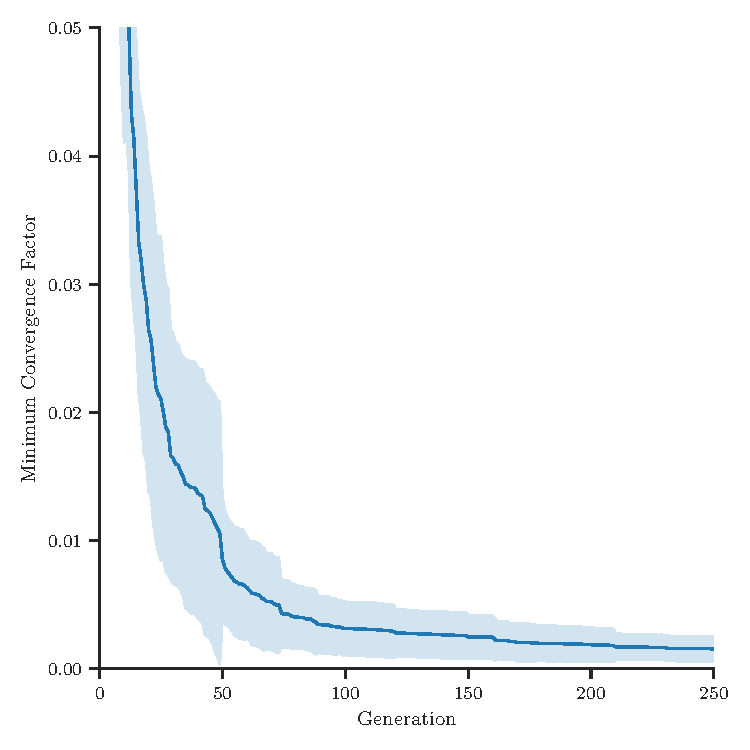
\includegraphics[width=\textwidth]{figures/minimum_convergence_factor_2D_FD_Poisson_fromL2.pdf}
		\caption{Minimum Convergence Factor}
		\label{fig:poisson-2D-minimum-convergence-factor}
	\end{subfigure}
	\hfill
	\begin{subfigure}[b]{0.49\textwidth}
		\centering
		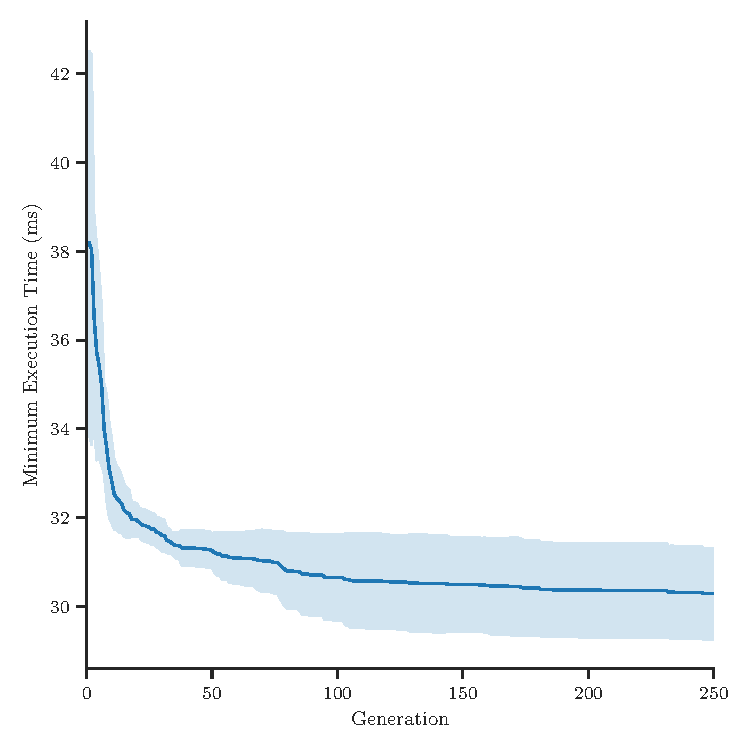
\includegraphics[width=\textwidth]{figures/minimum_execution_time_2D_FD_Poisson_fromL2.pdf}
		\caption{Minimum Execution Time per Iteration}
		\label{fig:poisson-2D-minimum-execution-time}
	\end{subfigure}
	\caption{2D Poisson - Mean and standard deviation of the minimum objective function values during the optimization.}
	\label{fig:poisson-2D-minimum-objectives}
\end{figure}
\begin{figure}
	\centering
	\begin{subfigure}[b]{0.49\textwidth}
		\centering
		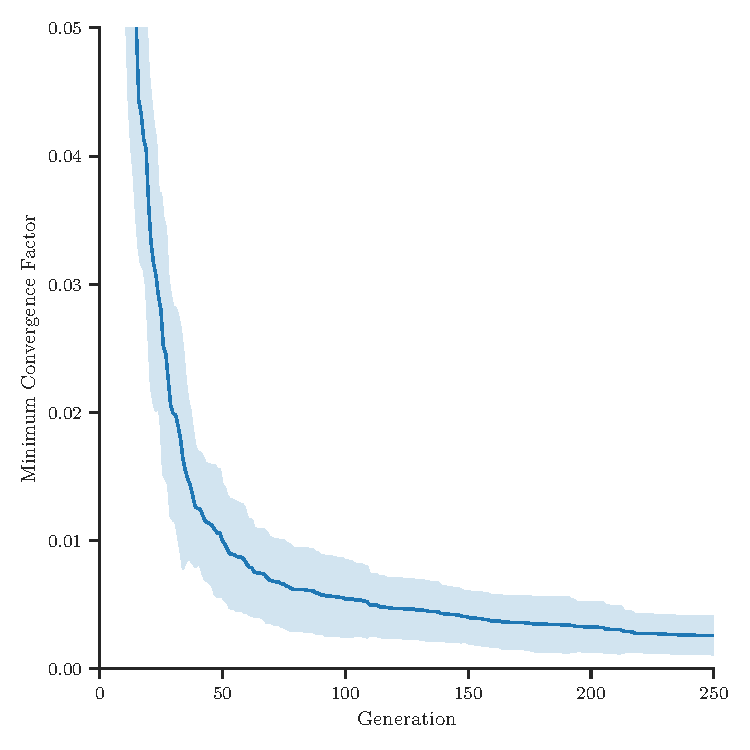
\includegraphics[width=\textwidth]{figures/minimum_convergence_factor_3D_FD_Poisson_fromL2.pdf}
		\caption{Minimum Convergence Factor}
		\label{fig:poisson-3D-minimum-convergence-factor}
	\end{subfigure}
	\hfill
	\begin{subfigure}[b]{0.49\textwidth}
		\centering
		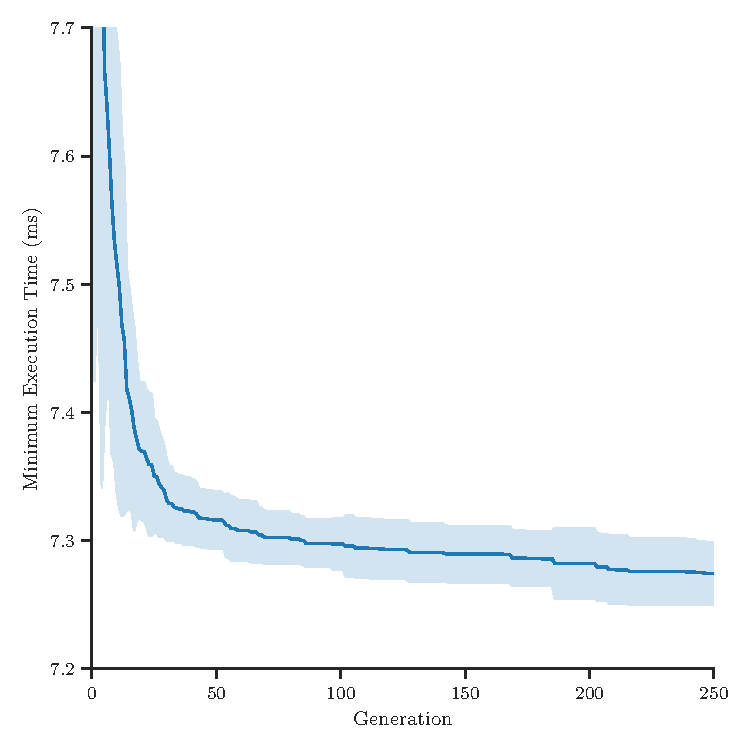
\includegraphics[width=\textwidth]{figures/minimum_execution_time_3D_FD_Poisson_fromL2.pdf}
		\caption{Minimum Execution Time per Iteration}
		\label{fig:poisson-3D-minimum-execution-time}
	\end{subfigure}
	\caption{3D Poisson - Mean and standard deviation of the minimum objective function values during the optimization.}
	\label{fig:poisson-3D-minimum-objectives}
\end{figure}
\begin{figure}
	\centering
	\begin{subfigure}[b]{0.49\textwidth}
		\centering
		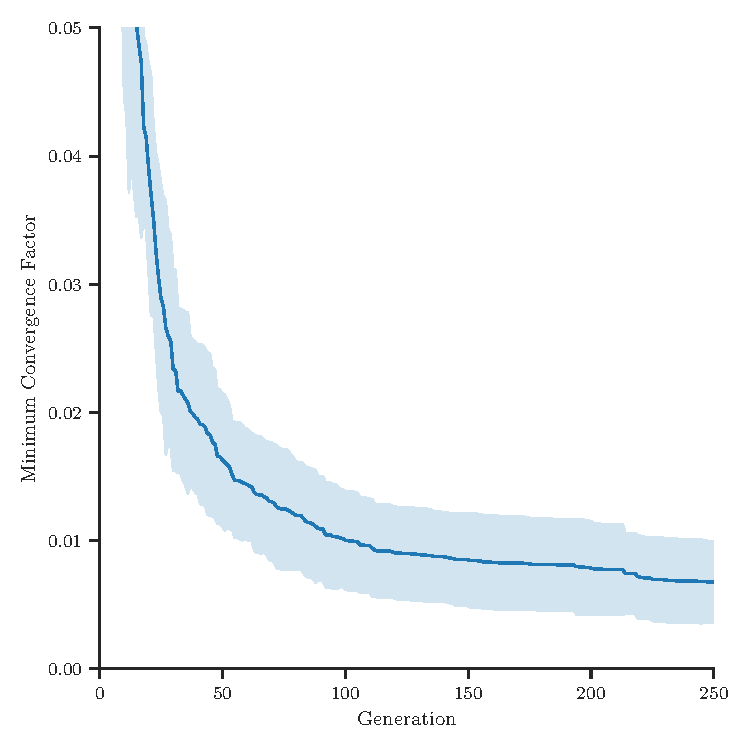
\includegraphics[width=\textwidth]{figures/minimum_convergence_factor_2D_FD_LinearElasticity_fromL2.pdf}
		\caption{Minimum Convergence Factor}
		\label{fig:linear-elasticity-2D-minimum-convergence-factor}
	\end{subfigure}
	\hfill
	\begin{subfigure}[b]{0.49\textwidth}
		\centering
		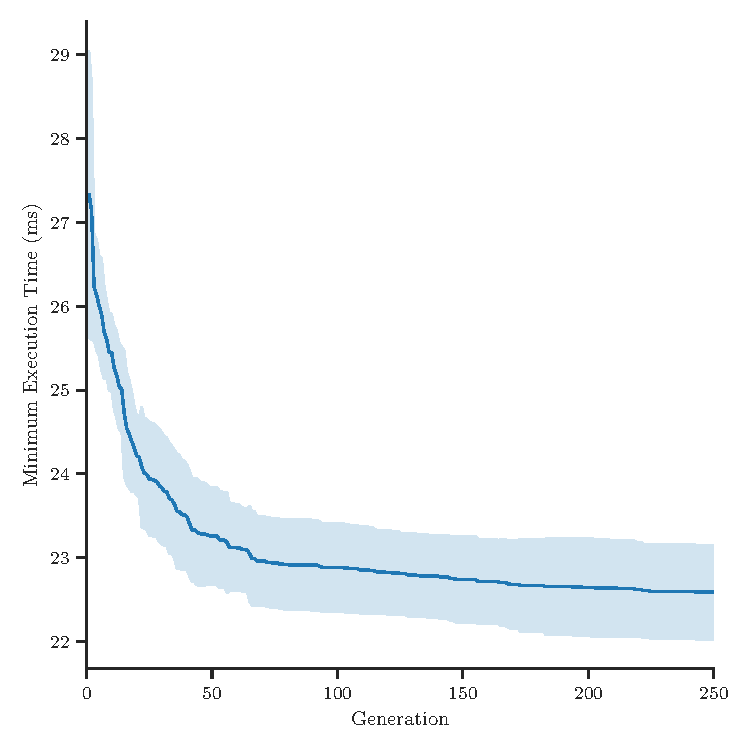
\includegraphics[width=\textwidth]{figures/minimum_execution_time_2D_FD_LinearElasticity_fromL2.pdf}
		\caption{Minimum Execution Time per Iteration}
		\label{fig:linear-elasticity-2D-minimum-execution-time}
	\end{subfigure}
	\caption{2D Linear Elasticity - Mean and standard deviation of the minimum objective function values during the optimization.}
	\label{fig:linear-elasticity-2D-minimum-objectives}
\end{figure}
First of all, we can conclude that in all three cases, our algorithm is able to quickly reduce the minimum value of both objectives within the population.
If we compare the slope of the two objectives for the three different problems, we can see that in the case of the first objective $\rho$, significantly more generations are required to achieve the same degree of reduction as for the second objective $t$.
However, the algorithm still significantly improves upon the current minimum of $\rho$ beyond the first 50 generations, which can be seen in Figure~\ref{fig:poisson-2D-minimum-convergence-factor},~\ref{fig:poisson-3D-minimum-convergence-factor} and~\ref{fig:linear-elasticity-2D-minimum-convergence-factor}.
For the second objective $t$, the majority of improvement happens within the first 50--70 generations, as it can be seen in Figure~\ref{fig:poisson-2D-minimum-execution-time},~\ref{fig:poisson-3D-minimum-execution-time} and~\ref{fig:linear-elasticity-2D-minimum-execution-time}.
Note that while the convergence factor is constant for each execution of the same solver, $t$ is obtained by measuring its execution time on the respective compute node.
Therefore, due to manufacturing and temperature-based variations, we can expect a certain degree of fluctuations when measuring the execution time of the same solver on different compute nodes during consecutive optimization runs.
Consequently, even though the algorithm is able to reduce the second objective faster, this effect induces a larger deviation between the individual experiments and, thus, an overall higher standard deviation.

Furthermore, by considering the absolute value of the minimum convergence factor attained in each of the three different cases, we can assess the difficulty of the underlying problem.
While the execution time per iteration $t$ is solely determined by the computational complexity of each solver and the properties of the given computer architecture, a smaller convergence factor indicates that the underlying problem is easier to solve.
Poisson's equation represents an often-studied model problem whose strong ellipticity enables its easy solution by multigrid~\cite{trottenberg2000multigrid}.
As a consequence, our method consistently discovers multigrid methods that achieve fast convergence, with minimum convergence factors of less than 0.005, for both the two and three-dimensional instances of this equation, which can be seen in Figure~\ref{fig:poisson-2D-minimum-convergence-factor} and~\ref{fig:poisson-3D-minimum-convergence-factor}.
In the case of the linear elastic boundary value problem, both the mean and standard deviation remain higher for the first objective throughout each experiment.
However, on average, our method is still able to discover multigrid methods that achieve a convergence factor of 0.01 or less, which equates to outstandingly fast convergence.
In summary, we can conclude that our evolutionary program synthesis method consistently yields multigrid cycles that represent satisfactory minima for both objectives in all three test cases considered.

To further analyze the behavior of our multi-objective evolutionary algorithm, we consider the distribution of non-dominated individuals at the end of all experiments, which is shown in Figure~\ref{fig:pareto-front-2D-poisson},~\ref{fig:pareto-front-3D-poisson} and~\ref{fig:pareto-front-2D-linear-elasticity}.
\begin{figure}
	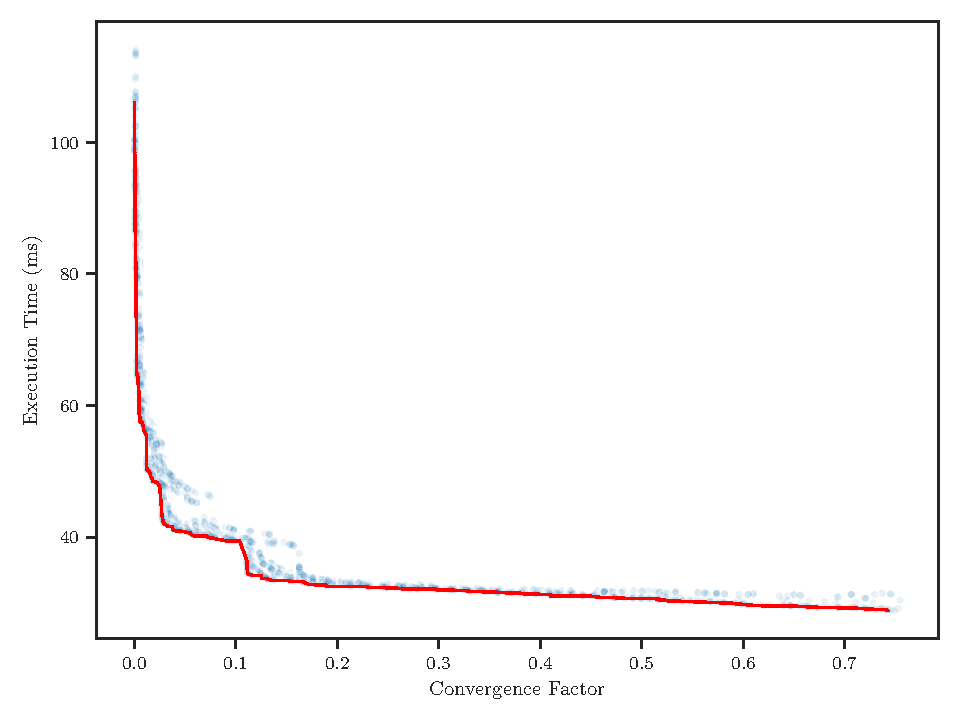
\includegraphics[width=\columnwidth]{figures/pareto_front_2D_FD_Poisson_fromL2.pdf}
	\caption{2D Poisson - Distribution of non-dominated individuals at the end of all ten experiments. The red line denotes the combined Pareto front.}
	\label{fig:pareto-front-2D-poisson}
\end{figure}
\begin{figure}
	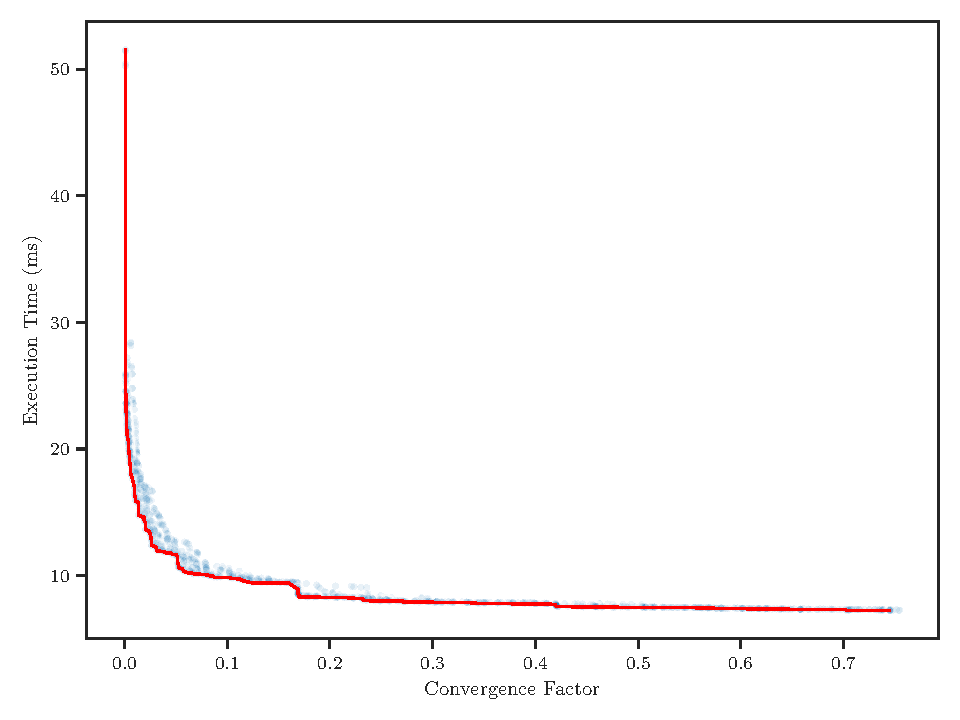
\includegraphics[width=\columnwidth]{figures/pareto_front_3D_FD_Poisson_fromL2.pdf}
	\caption{3D Poisson - Distribution of non-dominated individuals at the end of all ten experiments. The red line denotes the combined Pareto front.}
	\label{fig:pareto-front-3D-poisson}
\end{figure}
\begin{figure}
	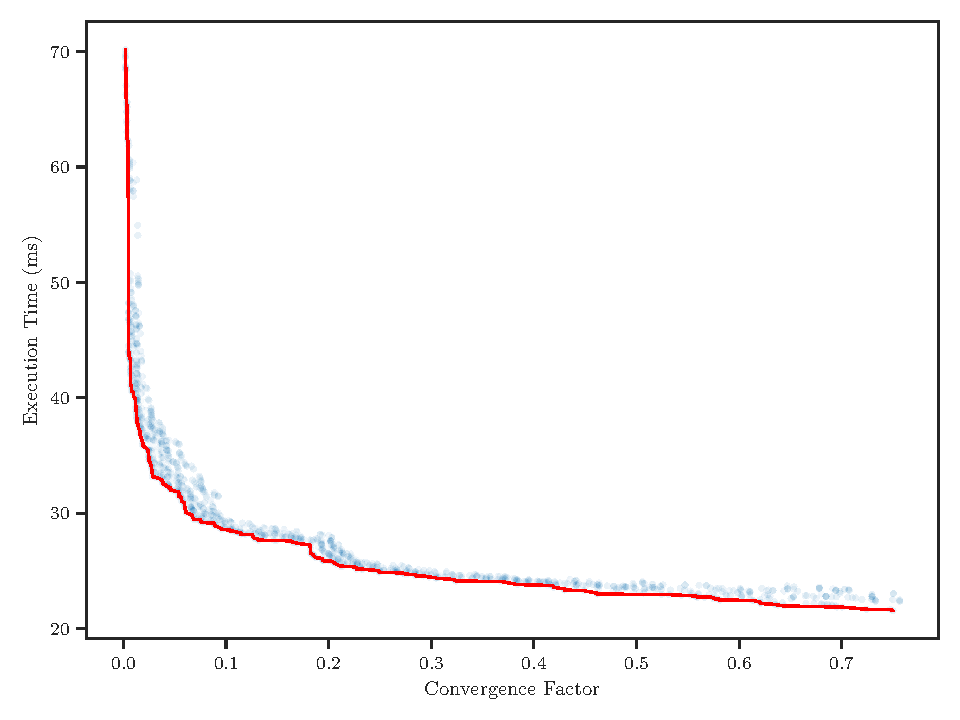
\includegraphics[width=\columnwidth]{figures/pareto_front_2D_FD_LinearElasticity_fromL2.pdf}
	\caption{2D Linear Elasticity - Distribution of non-dominated individuals at the end of all ten experiments. The red line denotes the combined Pareto front.}
	\label{fig:pareto-front-2D-linear-elasticity}
\end{figure}
Here the red line denotes the combined front, while the color density of the distribution indicates where most of the solutions are located at the end of all experiments. 
In all three cases, the majority of non-dominated solutions obtained within each experiment can be found close to the combined front.
While in Figure~\ref{fig:pareto-front-2D-poisson}, the number of solutions that are distinctly located outside of the front is slightly higher than in the other two cases, their distance to the red line is still comparably small compared to the complete objective space.
Again we can attribute part of this effect to variations in the execution time on different compute nodes.
Furthermore, note that throughout most of the objective space, but especially in the center, the solutions are evenly distributed alongside the front.
Here only the left-upper part of Figure~\ref{fig:pareto-front-3D-poisson} and~\ref{fig:pareto-front-2D-linear-elasticity} represents a noteworthy exception, where our approach struggles to discover the same solutions within each experiment.
An explanation for this effect is that the solutions located in this part of the space are characterized by an extremely fast convergence.
Since the convergence of a multigrid method can primarily be accelerated with the addition of smoothing and coarse-grid correction steps, discovering the same non-dominated solutions with fast convergence requires us to construct the same large expressions starting from different random initializations.
Recently, the impaired capabilities of NSGA-II to evolve large non-dominated expressions have been demonstrated in~\cite{liu2022evolvability}, which similarly explains why our implementation struggles to consistently discover the same fast-converging solutions.

\subsection{Comparison with Reference Methods}
Finally, in order to investigate whether our evolutionary program synthesis method yields multigrid methods that are competitive with well-known multigrid cycles, we consider two different multi-core CPU architectures for evaluation: Intel Xeon E5-2630v4 (Broadwell) and Intel Xeon 2660v2 (Ivy Bridge).
In both cases, each compute node consists of two sockets with 20 physical CPU cores and a cache-coherent NUMA architecture.
In order to assess the solving speed of the methods evolved, we consider two different problem sizes for each of the three test cases.
While in the first case, a problem size identical to the one employed within the evolutionary search is chosen, in the second case, we obtain a larger one by doubling the number of grid points in each dimension.
To measure the solving speed of each method, we execute it on a dedicated node using a thread-based parallelization with 20 OpenMP threads, whereby we pin each thread to a unique physical core and employ the same parallelization approach as described in Section~\ref{sec:optimization-settings}.
Even though the evaluation of generalizability is not the focus of this section, it is still worthwhile to investigate whether the methods discovered with our approach are capable of solving larger instances of the same problem.
For comparison, we consider a number of different V-cycles with at most four RB-GS pre and post-smoothing steps.
With the exception of full-multigrid (FMG) methods, which require a different formulation than the one considered here, these cycles are known to be the fastest multigrid-based solvers for Poisson's equation~\cite{trottenberg2000multigrid}.
As we have already investigated in~\cite{schmitt2020constructing}, the same is true for the linear elastic boundary value problem considered here.
To achieve a fair comparison, we empirically choose the optimum relaxation factor $\omega$ for each test case from the same interval considered within our experiments, which leads to $\omega = 1.15$ for the two-dimensional Poisson equation and $\omega = 1.25$ both for the three-dimensional Poisson equation and the linear elastic boundary value problem.
Table~\ref{table:poisson-2D-reference-methods},~\ref{table:poisson-3D-reference-methods} and~\ref{table:linear-elasticity-2D-reference-methods} contains the resulting solving times and the number of iterations required to achieve the desired defect reduction for the respective test case.
Here, for instance, the abbreviation V(2,1) denotes a V-cycle with two pre and one post-smoothing step with RB-GS.
First of all, as we can expect from a functioning multigrid method, the number of iterations stays constant for both problem sizes, only with the exception of the V(1,0)-cycle, where we can observe a slight increase for the linear elastic boundary value problem.
Overall, we can conclude that while the V(2,2)-cycle represents the fastest solver for both cases of Poisson's equation, the V(3,3) cycle leads to the fastest solving time for the linear elastic boundary value problem.
\begin{table}
	\caption{2D Poisson - Measured number of iterations and solving times of the reference methods on 20 cores and two sockets.}
	\label{table:poisson-2D-reference-methods}
	\centering
	\begin{tabular}{l c c c c c c}
		\toprule
		& \multicolumn{2}{c}{Iterations} & \multicolumn{2}{c}{Broadwell (ms)} & \multicolumn{2}{c}{Ivy Bridge (ms)} \\
		\cmidrule(r){2-3} \cmidrule(r){4-5} \cmidrule(r){6-7}
		$l_{max}$ & $11$& $12$ & $11$ & $12$ & $11$ & $12$\\
		\midrule
		V(1, 0) & 21 & 21 & 969 & 2810 & 879 & 2652 \\
		\midrule
		V(1, 1) & 9 & 9 & 461 & 1359 & 411 & 1287 \\
		\midrule
		V(2, 1) & 7 & 7 & 377 & 1137 & 334 & 1087\\
		\midrule
		V(2, 2) & 6 & 6 & 344 & 1056 & 302 & 1007 \\
		\midrule
		V(3, 2) & 6 & 6 & 378 & 1160 & 324 & 1112 \\
		\midrule
		V(3, 3) & 6 & 6 & 397 & 1255 & 344 & 1201 \\
		\midrule
		V(4, 3) & 6 & 6 & 425 & 1350 & 366 & 1306 \\
		\midrule
		V(4, 4) & 6 & 6 & 448 & 1449 & 383 & 1409\\
		\bottomrule
	\end{tabular}
	%FMG for max_level = 12: 530.3038500000001 ms, 3 Iterations
\end{table}
\begin{table}
	\caption{3D Poisson - Measured number of iterations and solving times of the reference methods on 20 cores and two sockets.}
	\label{table:poisson-3D-reference-methods}
	\centering
	\begin{tabular}{l c c c c c c}
		\toprule
		& \multicolumn{2}{c}{Iterations} & \multicolumn{2}{c}{Broadwell (ms)} & \multicolumn{2}{c}{Ivy Bridge (ms)} \\
		\cmidrule(r){2-3} \cmidrule(r){4-5} \cmidrule(r){6-7}
		$l_{max}$ & $7$& $8$ & $7$ & $8$ & $7$ & $8$\\
		\midrule
		V(1, 0) & 29 & 30 & 121.3 &1221 & 134.6 & 1470 \\
		\midrule
		V(1, 1) & 13 & 13 & 70.8 & 682 & 79.9 & 838 \\
		\midrule
		V(2, 1) & 9 & 9 & 59.0 & 582 & 66.2 & 708 \\
		\midrule
		V(2, 2) & 7 & 7 & 54.6 & 531 & 65.4 & 654 \\
		\midrule
		V(3, 2) & 7 & 7 & 61.9 & 610 & 74.6 & 757 \\
		\midrule
		V(3, 3) & 7 & 7 & 72.6 & 690 & 86.6 & 857 \\
		\midrule
		V(4, 3) & 7 & 6 & 77.9 & 656 & 87.3 & 825 \\
		\midrule
		V(4, 4) & 6 & 6 & 73.2 & 725 & 82.5 & 906 \\
		\bottomrule
	\end{tabular}
\end{table}
\begin{table}
	\caption{2D Linear Elasticity - Measured number of iterations and solving times of the reference methods on 20 cores and two sockets.}
	\label{table:linear-elasticity-2D-reference-methods}
	\centering
	\begin{tabular}{l c c c c c c}
		\toprule
		& \multicolumn{2}{c}{Iterations} & \multicolumn{2}{c}{Broadwell (ms)} & \multicolumn{2}{c}{Ivy Bridge (ms)} \\
		\cmidrule(r){2-3} \cmidrule(r){4-5} \cmidrule(r){6-7}
		$l_{max}$ & $10$& $11$ & $10$ & $11$ & $10$ & $11$\\
		\midrule
		V(1, 0) & 32 & 31 & 872 & 4306 & 828 & 4128 \\
		\midrule
		V(1, 1) & 15 & 15 & 439 & 2118 & 418 & 2075\\
		\midrule
		V(2, 1) & 10 & 10 & 318 & 1529 & 312 & 1529 \\
		\midrule
		V(2, 2) & 9 & 9 & 314 & 1449 & 316 & 1476 \\
		\midrule
		V(3, 2) & 8 & 8 & 297 & 1368 & 304 & 1388 \\
		\midrule
		V(3, 3) & 7 & 7 & 283 & 1247 & 288 & 1288 \\
		\midrule
		V(4, 3) & 7 & 7 & 293 & 1320 & 313 & 1397 \\
		\midrule
		V(4, 4) & 7 & 7 & 311 & 1378 & 334 & 1471 \\
		\bottomrule
	\end{tabular}
\end{table}

Finally, we evaluate the multigrid methods obtained with our evolutionary program synthesis method in each of the ten experiments under the same conditions.
As the number of non-dominated individuals within the population at the end of each experiment is unrestricted and can, therefore, be too high for a direct evaluation, we heuristically identify the 50 most promising individuals by sorting them according to the metric
\begin{equation}
	T_{\varepsilon} = \frac{\log(\varepsilon)}{\log(\rho)} \cdot t,
\end{equation}
where $\varepsilon = 10^{-12}$ is the desired defect reduction factor and $\rho$ and $t$ the attained objective function values.
Each of the resulting multigrid methods is then executed as a solver for the respective test problem on a Broadwell compute node consisting of two sockets with 20 CPU cores, whereby we employ the same problem size as within each experiment.
Note that while both the problem size and computer architecture are identical, increasing the number of CPU cores leads to a higher degree of parallelism and, thus, a smaller execution time per iteration.
After we have identified the method that leads to the fastest solver in each case, we execute it on both problem sizes and evaluation platforms, as described above.
Table~\ref{table:poisson-2D-evolved-methods},~\ref{table:poisson-3D-evolved-methods} and~\ref{table:linear-elasticity-2D-evolved-methods} contain the resulting measured solving times for each case.
\begin{table}
	\caption{2D Poisson - Measured number of iterations and solving times of the evolved multigrid methods on 20 cores and two sockets.}
	\label{table:poisson-2D-evolved-methods}
	\centering
	\begin{tabular}{l c c c c c c}
		\toprule
		& \multicolumn{2}{c}{Iterations} & \multicolumn{2}{c}{Broadwell (ms)} & \multicolumn{2}{c}{Ivy Bridge (ms)} \\
		\cmidrule(r){2-3} \cmidrule(r){4-5} \cmidrule(r){6-7}
		$l_{max}$ & $11$& $12$ & $11$ & $12$ & $11$ & $12$\\
		\midrule
		ES-1 & 5 & 5 & 338 & 1064 & 304 & 1055\\
		\midrule
		ES-2 & 6 & 6 & 371 & 1163 & 330 & 1133 \\
		\midrule
		ES-3 & 5 & 5 & 311 & 988 & 279 & 976 \\
		\midrule
		ES-4 & 6 & 6 & 380 & 1188 & 338 & 1153 \\
		\midrule
		ES-5 & 5 & 5 & 312 & 978 & 279 & 963 \\
		\midrule
		ES-6 & 5 & 5 & 349 & 1123 & 309 & 1106 \\
		\midrule
		ES-7 & 6 & 6 & 354 & 1096 & 320 & 1068 \\
		\midrule
		ES-8 & 6 & 6 & 347 & 1081 & 310 & 1056 \\
		\midrule
		ES-9 & 6 & 6 & 353 & 1079 & 313 & 1045 \\
		\midrule
		ES-10 & 5 & 5 & 310 & 960 & 275 & 934 \\
		\bottomrule
	\end{tabular}
\end{table}
\begin{table}
	\caption{3D Poisson - Measured number of iterations and solving times of the evolved multigrid methods on 20 cores and two sockets.}
	\label{table:poisson-3D-evolved-methods}
	\centering
	\begin{tabular}{l c c c c c c}
		\toprule
		& \multicolumn{2}{c}{Iterations} & \multicolumn{2}{c}{Broadwell (ms)} & \multicolumn{2}{c}{Ivy Bridge (ms)} \\
		\cmidrule(r){2-3} \cmidrule(r){4-5} \cmidrule(r){6-7}
		$l_{max}$ & $7$& $8$ & $7$ & $8$ & $7$ & $8$\\
		\midrule
		ES-1 & 10 & 11 & 55.3 & 577 & 70.0 & 704\\
		\midrule
		ES-2 & 8 & 9 & 57.2 & 578 & 64.3 & 716 \\
		\midrule
		ES-3 & 8 & 9 & 59.0 & 671 & 65.3 & 824 \\
		\midrule
		ES-4 & 8 & 9 & 54.6 & 576 & 62.7 & 710 \\
		\midrule
		ES-5 & 8 & 10 & 54.6 & 641 & 60.9 & 789 \\
		\midrule
		ES-6 & 9 & 10 & 59.4 & 716 & 67.1 & 891 \\
		\midrule
		ES-7 & 6 & 8 & 56.2 & 702 & 70.9 & 880 \\
		\midrule
		ES-8 & 5 & 5 & 56.7 & 589 & 74.0 & 724 \\
		\midrule
		ES-9 & 10 & 10 & 61.0 & 568 & 66.3 & 681 \\
		\midrule
		ES-10 & 10 & 11 & 55.4 & 581 & 61.3 & 705 \\
		\bottomrule
	\end{tabular}
\end{table}
\begin{table}
	\caption{2D Linear Elasticity - Measured number of iterations and solving times of the evolved multigrid methods on 20 cores and two sockets.}
	\label{table:linear-elasticity-2D-evolved-methods}
	\centering
	\begin{tabular}{l c c c c c c}
		\toprule
		& \multicolumn{2}{c}{Iterations} & \multicolumn{2}{c}{Broadwell (ms)} & \multicolumn{2}{c}{Ivy Bridge (ms)} \\
		\cmidrule(r){2-3} \cmidrule(r){4-5} \cmidrule(r){6-7}
		$l_{max}$ & $10$& $11$ & $10$ & $11$ & $10$ & $11$\\
		\midrule
		ES-1 & 6 & 6 & 234 & 1117 & 235 & 1137 \\
		\midrule
		ES-2 & 6 & 6 & 216 & 1033 & 211 & 1035 \\
		\midrule
		ES-3 & 7 & 7 & 258 & 1225 & 259 & 1231 \\
		\midrule
		ES-4 & 6 & 6 & 226 & 1077 & 219 & 1093 \\
		\midrule
		ES-5 & 6 & 6 & 235 & 1121 & 229 & 1139 \\
		\midrule
		ES-6 & 6 & 6 & 220 & 1083 & 213 & 1093 \\
		\midrule
		ES-7 & 7 & 7 & 238 & 1191 & 236 & 1186 \\
		\midrule
		ES-8 & 6 & 6 & 217 & 1037 & 223 & 1039 \\
		\midrule
		ES-9 & 6 & 6 & 224 & 1039 & 222 & 1058 \\
		\midrule
		ES-10 & 7 & 7 & 243 & 1188 & 238 & 1188 \\
		\bottomrule
	\end{tabular}
\end{table}
In general, we can conclude that in all three cases, our evolutionary program synthesis method was consistently able to discover well-functioning multigrid methods, leading to fast solving times for both problem sizes.
Furthermore, in the case of the two-dimensional Poisson equation and linear elasticity, our approach yields multigrid methods that achieve an even higher error reduction efficiency than the best reference cycle.
Here, the fastest discovered method for the two-dimensional Poisson equation, ES-10, leads to a $9 \%$ solving time improvement compared to the V(2,2)-cycle on both architectures, while for linear elasticity the ES-2 method achieves an even larger speedup of 17--27 \% compared to the V(3,3)-cycle.
%Interestingly, in contrast to the other two cases, for the two-dimensional Poisson equation, all solvers achieve faster execution times on the older Ivy Bridge computer architecture.
%Further investigating this phenomenon would require us to perform an in-depth analysis of the generated code.
%However, since our focus is a comparison of the relative performance of different multigrid methods on the same architecture, we have not yet performed such an analysis.
While in the case of the three-dimensional Poisson, the methods discovered with our approach still represent competitive solvers, they are not able to achieve the same degree of efficiency in solving both problem sizes.
In particular, with the exception of the ES-8 and ES-9 methods, we observe a slight increase in the number of iterations for the larger instance of this problem, which leads to a larger increase in the solving times compared to the reference cycles.
This effect indicates that not all multigrid methods obtained for a particular instance of this test problem can be generalized to larger problem instances without further adaption.
In Section~\ref{sec:generalization}, we have already addressed this issue by proposing a multigrid-specific generalization scheme, whose effectiveness will be investigated in the next section of this chapter.   
%we have already presented an adapted version of our multi-objective evolutionary algorithm that aims to overcome these limitations by iteratively increasing the problem size during the search.
%In the next section of this chapter, we will, thus, investigate the effectiveness of this approach on the indefinite Helmholtz equation, a problem of substantially higher difficulty than those considered within this section.

To conclude our experimental analysis, Figure~\ref{fig:evolved-methods-graphical-representation:2D} and~\ref{fig:evolved-methods-graphical-representation:3D} contains a graphical representation of the discovered multigrid method that achieves the fastest solving time for the larger problem instance of two and three-dimensional Poisson equation, respectively. 
\begin{figure}
	%2D Poisson
 \captionsetup[subfigure]{justification=centering}
		\begin{subfigure}[b]{\columnwidth}
			\scalebox{0.75}{%
			\begin{tikzpicture}
				\node   (h) at (-0.75, 4){$h$};
				\node   (2h) at (-0.75, 3){$2h$};
				\node   (4h) at (-0.75, 2){$4h$};
				\node   (8h) at (-0.75, 1){$8h$};
				\node   (16h) at (-0.75, 0){$16h$};
				\node	(a) at (0,4) [draw, fill=lightred, circle,inner sep=0pt,minimum size=5mm] {\tiny $1.15$};
				\node	(b) at (0.5,3) [draw, circle,inner sep=0pt,minimum size=5mm] {\phantom{\tiny $1.00$}};
				\node	(c) at (1,2) [draw, circle,fill=lightred,inner sep=0pt,minimum size=5mm] {\tiny $0.80$};
				\node	(d) at (1.5,1) [draw, circle,inner sep=0pt,minimum size=5mm] {\phantom{\tiny $1.00$}};
				\node	(e) at (2,0) [draw, circle,fill=black, inner sep=0pt,minimum size=5mm] {\phantom{\tiny $1.00$}};
				\node	(f) at (2.5,1) [draw, circle,  fill=lightred,inner sep=0pt,minimum size=5mm] {\tiny $1.90$};
				\node	(g) at (3,2) [draw, circle,fill=lightred,inner sep=0pt,minimum size=5mm] {\tiny $1.40$};
				\node	(h) at (4,2) [draw, circle,fill=lightred,inner sep=0pt,minimum size=5mm] {\tiny $1.65$};
				\node	(i) at (5,2) [draw, circle,fill=lightred,inner sep=0pt,minimum size=5mm] {\tiny $1.45$};
				\node	(j) at (6,2) [draw, circle,fill=lightred,inner sep=0pt,minimum size=5mm] {\tiny $1.05$};
				\node	(k) at (6.5,3) [draw, circle,fill=lightred,inner sep=0pt,minimum size=5mm] {\tiny $1.30$};
				\node	(l) at (7.5,3) [draw, circle,fill=lightred,inner sep=0pt,minimum size=5mm] {\tiny $0.55$};
				\node	(m) at (8,4) [draw, circle,fill=lightred,inner sep=0pt,minimum size=5mm] {\tiny $1.05$};
				\node	(n) at (9,4) [draw, circle,fill=lightred,inner sep=0pt,minimum size=5mm] {\tiny $1.05$};
				\node	(o) at (9.5,3) [draw, circle, inner sep=0pt,minimum size=5mm] {\phantom{\tiny $1.00$}};
				\node	(p) at (10,2) [draw, circle, inner sep=0pt,minimum size=5mm] {\phantom{\tiny $1.00$}};
				\node	(q) at (10.5,1) [draw, circle, fill=lightred, inner sep=0pt,minimum size=5mm] {\tiny $0.90$};
				\node	(r) at (11.5,1) [draw, circle, fill=lightred, inner sep=0pt,minimum size=5mm] {\tiny $1.40$};
				\node	(s) at (12,2) [draw, circle, fill=lightred, inner sep=0pt,minimum size=5mm] {\tiny $0.95$};
				\node	(t) at (13,2) [draw, circle, fill=lightred, inner sep=0pt,minimum size=5mm] {\tiny $1.25$};
				\node	(u) at (14,2) [draw, circle, fill=lightred, inner sep=0pt,minimum size=5mm] {\tiny $1.05$};
				\node	(v) at (14.5,3) [draw, circle, fill=lightred, inner sep=0pt,minimum size=5mm] {\tiny $1.00$};
				\node	(w) at (15,4) [draw, circle, fill=lightred, inner sep=0pt,minimum size=5mm] {\tiny $1.05$};
				\draw 
				(a) edge[->] (b) 
				(b) edge[->] (c)
				(c) edge[->] (d)
				(d) edge[->] (e)   
				(e) edge[->] node[near end,left] {\tiny 0.80} (f)
				(f) edge[->] node[near end,left] {\tiny 1.20} (g)
				(g) edge[->] (h)
				(h) edge[->] (i)
				(i) edge[->] (j) 
				(j) edge[->] node[near end,left] {\tiny 0.90} (k)
				(k) edge[->] (l)
				(l) edge[->] node[near end,left] {\tiny 1.15} (m)   
				(m) edge[->] (n)
				(n) edge[->] (o)
				(o) edge[->] (p)
				(p) edge[->] (q)
				(q) edge[->] (r)
				(r) edge[->] node[near end,left] {\tiny 1.20} (s)
				(s) edge[->] (t)
				(t) edge[->] (u)
				(u) edge[->] node[near end,left] {\tiny 0.90} (v)
				(v) edge[->] node[near end,left] {\tiny 1.30} (w)
				;
			\end{tikzpicture}
		}
	\caption{2D Poisson: ES-10}
	\label{fig:evolved-methods-graphical-representation:2D}
	\end{subfigure}
  \par\bigskip
	\begin{subfigure}[b]{\columnwidth}
	\scalebox{0.75}{%
		\begin{tikzpicture}
			\node   (h) at (-0.75, 4){$h$};
			\node   (2h) at (-0.75, 3){$2h$};
			\node   (4h) at (-0.75, 2){$4h$};
			\node   (8h) at (-0.75, 1){$8h$};
			\node   (16h) at (-0.75, 0){$16h$};
			\node	(a) at (0,4) [draw, circle,inner sep=0pt,minimum size=5mm] {\phantom{\tiny $1.00$}};
			\node	(b) at (0.5,3) [draw, circle, fill=lightred, inner sep=0pt,minimum size=5mm] {\tiny $1.30$};
			\node	(c) at (1,2) [draw, circle,inner sep=0pt,minimum size=5mm] {\phantom{\tiny $1.00$}};
			\node	(d) at (1.5,1) [draw, circle,fill=lightred, inner sep=0pt,minimum size=5mm] {\tiny $0.85$};
			\node	(e) at (2,0) [draw, circle,fill=black, inner sep=0pt,minimum size=5mm] {\phantom{\tiny $1.00$}};
			\node	(f) at (2.5,1) [draw, circle,inner sep=0pt,minimum size=5mm] {\phantom{\tiny $1.00$}};
			\node	(g) at (3,2) [draw, circle,fill=lightblue,inner sep=0pt,minimum size=5mm, label=above:{\tiny $(2,1,1)$}] {\tiny 1.00}; %TODO add block info
			\node	(h) at (4,2) [draw, circle,fill=lightblue,inner sep=0pt,minimum size=5mm] {\tiny $1.5$};
			\node	(i) at (5,2) [draw, circle,fill=lightred,inner sep=0pt,minimum size=5mm] {\tiny $1.85$};
			\node	(j) at (6,2) [draw, circle,fill=lightred,inner sep=0pt,minimum size=5mm] {\tiny $0.75$};
			\node	(k) at (7,2) [draw, circle,fill=lightblue,inner sep=0pt,minimum size=5mm] {\tiny $0.60$};
			\node	(l) at (8,2) [draw, circle,fill=lightred,inner sep=0pt,minimum size=5mm] {\tiny $0.85$};
			\node	(m) at (8.5,1) [draw, circle,fill=lightred,inner sep=0pt,minimum size=5mm] {\tiny $0.85$};
			\node	(n) at (9,0) [draw, circle,fill=black,inner sep=0pt,minimum size=5mm] {\phantom{\tiny $1.00$}};
			\node	(o) at (9.5,1) [draw, circle,inner sep=0pt,minimum size=5mm] {\phantom{\tiny $1.00$}};
			\node	(p) at (10,2) [draw, circle,  fill=lightred, inner sep=0pt,minimum size=5mm] {\tiny $1.55$};
			\node	(q) at (10.5,3) [draw, circle, fill=lightred, inner sep=0pt,minimum size=5mm] {\tiny $1.30$};
			\node	(r) at (11,4) [draw, circle, fill=lightred, inner sep=0pt,minimum size=5mm] {\tiny $1.05$};
			\node	(s) at (12,4) [draw, circle, fill=lightred, inner sep=0pt,minimum size=5mm] {\tiny $1.25$};
			\draw 
			(a) edge[->] (b) 
			(b) edge[->] (c)
			(c) edge[->] (d)
			(d) edge[->] (e)   
			(e) edge[->] node[near end,left] {\tiny 0.80} (f)
			(f) edge[->] node[near end,left] {\tiny 1.20} (g)
			(g) edge[->] (h)
			(h) edge[->] (i)
			(i) edge[->] (j) 
			(j) edge[->] (k)
			(k) edge[->] (l)
			(l) edge[->] (m)   
			(m) edge[->] (n)
			(n) edge[->] node[near end,left] {\tiny 0.85}(o)
			(o) edge[->] node[near end,left] {\tiny 1.00}(p)
			(p) edge[->] node[near end,left] {\tiny 1.30}(q)
			(q) edge[->] node[near end,left] {\tiny 0.90}(r)
			(r) edge[->] (s)
			;
		\end{tikzpicture}
	}
	\caption{3D Poisson: ES-9}
	\label{fig:evolved-methods-graphical-representation:3D}
	\end{subfigure}
	\caption{Computational structure of the evolved multigrid methods. The color of the node denotes the type of operation. Black: Coarse-grid solver, Blue: Block Jacobi smoothing, Red: Red-black Gauss-Seidel smoothing, White: No operation. The relaxation factor of each smoothing step is included in each node, while for coarse-grid correction, it is attached to the respective edge. For block smoothers, the dimension of the block is specified on top of the respective node. If no block size is specified, pointwise smoothing is applied.}
	\label{fig:evolved-methods-graphical-representation}
\end{figure}
The first observation that can be made from investigating the computational structure of these methods is that none of them can be clearly characterized as a V-, F- or W-cycle.
It is, therefore, impossible to formulate each of them within the framework of classical multigrid cycles, as shown in Algorithm~\ref{alg:multigrid-cycle}.
While, for instance, the first part of Figure~\ref{fig:evolved-methods-graphical-representation:2D} can be characterized as a V-cycle, the method then proceeds with an additional coarse-grid correction step that is based on a purely smoothing-based error reduction on the coarser levels.
Figure~\ref{fig:evolved-methods-graphical-representation:3D} starts off in a similar fashion but then applies an additional three-grid V-cycle on the third-finest level with a step size of $4h$, before it transfers the computed correction back to the finest level.
The analysis performed in the recent work by Avnat and Yavneh already suggests that employing cycles of non-classical structure can lead to a significantly higher degree of efficiency in solving certain PDEs~\cite{avnat2022recursive}. 
However, in addition to their non-classical structure, both multigrid methods employ a different number of smoothings steps on each level using a wide range of different relaxation factors, whereby, in general, on certain levels, significantly more smoothing is performed than on others.
In particular, smoothing on the third-finest level seems to be exceptionally effective in reducing the most significant error components, and hence, the number of smoothing steps on this level is higher than on any other level.
While both methods predominantly employ RB-GS as a smoother, Figure~\ref{fig:evolved-methods-graphical-representation:3D} also includes individual pointwise and block Jacobi steps.
Finally, the even more complicated computational structure of the methods discovered for the linear elastic boundary prevents us from including their graphical representations similar to Figure~\ref{fig:evolved-methods-graphical-representation}.
However, if we consider the evolved method ES-2, which leads to the fastest solving time for the larger instance of the linear elastic boundary value problem with $l_{max} = 11$, we can observe a number of structural similarities with the methods shown in Figure~\ref{fig:evolved-methods-graphical-representation}.
In particular, the method applies the coarse-grid solver only once within its computations and, therefore, resembles a V-cycle but also includes additional smoothing-based coarse-grid correction steps with a varying amount of smoothing on each level.
Furthermore, with the exception of a single Jacobi step on the second-coarsest level, the method employs exclusively RB-GS smoothing.

\section{Discovering Generalizable Multigrid-Based Preconditioners for the Helmholtz Equation}
While within the last section, we could already demonstrate that our evolutionary program synthesis approach leads to the automated design of multigrid methods with competitive performance compared to common multigrid cycles, none of the PDEs considered there is particularly challenging to solve.   
Therefore, in order to evaluate whether our approach can achieve any advantages compared to state-of-the-art methods in the case of a problem that is difficult to solve numerically, we consider the indefinite Helmholtz equation.
At this point, we would like to point out that all results presented in this section have been originally published in~\cite{schmitt2022evolving}.
The Helmholtz equation, whose basic form is given as 
\begin{equation}
	-\nabla ^{2}u - k^{2}u = f,
	\label{eq:helmholtz}
\end{equation} 
is a famously-difficult test problem for the application of numerical methods that also has practical relevance for many real-world applications, such as~\cite{versteeg1994marmousi,martin2006marmousi2,billette20052004,gray1995migration}.
The main difficulty in solving this equation is that the system of linear equations resulting from its discretization becomes highly ill-conditioned for large values of the wavenumber $k$~\cite{ernst2012difficult}.
If we, for instance, assume the use of ten grid points per wavelength\footnote{Usually the relation of the wavelength $\lambda$ to the wavenumber $k$ is defined as $k = 2 \pi/\lambda$ }, as it is common in geophysical applications~\cite{erlangga2006multigrid}, on the dimensionless unit square, a second-order accuracy requirement of $kh = 0.625$ must be fulfilled.
Figure~\ref{fig:condition-number-helmholtz} shows the condition number of the system matrix $A$ that results from a discretization of Equation~\eqref{eq:helmholtz} for different values of the wavenumber $k$.
\begin{figure}
		\centering
		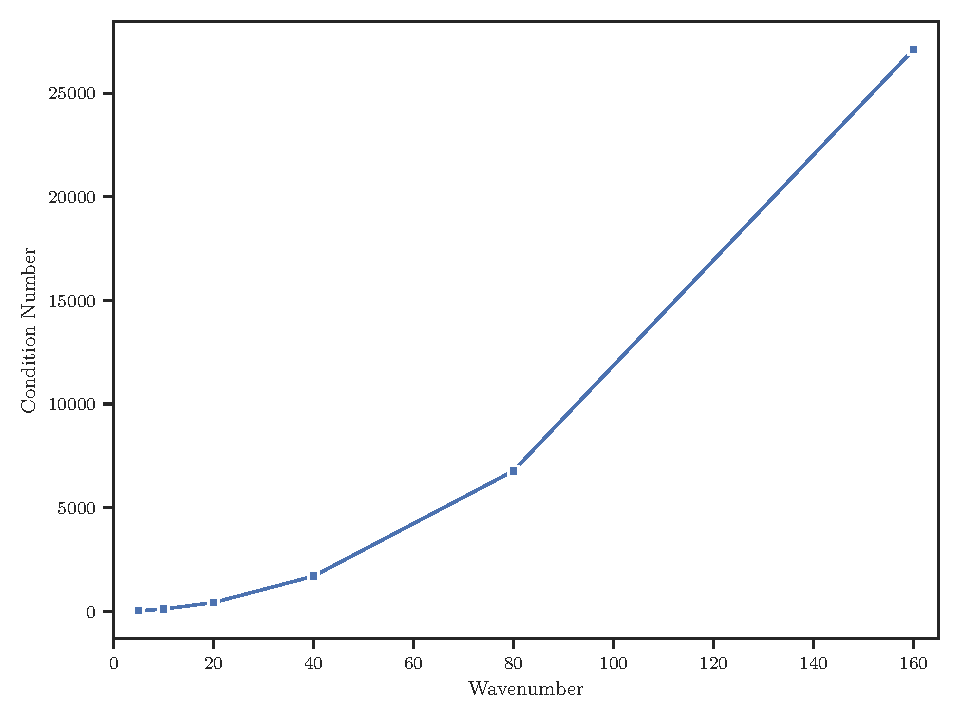
\includegraphics[width=\textwidth]{figures/cond.pdf}
		\caption{Condition number of the system matrix resulting from a finite-difference discretization of the two-dimensional Helmholtz equation with $kh = 0.625$}
		\label{fig:condition-number-helmholtz}
\end{figure}
The condition number gives us a measure of how much an initial approximation error is magnified by the application of the operator $A$.
As we can see in Figure~\ref{fig:condition-number-helmholtz} for larger values of $k$, the condition number of $A$ increases dramatically, which leads to an extreme accumulation of numerical errors. 
The necessity to handle these errors makes the design of an efficient or even functioning numerical method for the indefinite Helmholtz equation outstandingly difficult.
In particular, without any modification, classical multigrid methods can not effectively be applied as a numerical solver for indefinite Helmholtz problems~\cite{ernst2012difficult}.
One multigrid-based approach that mitigates this problem is the application of the method as a preconditioner instead of applying it to the discretized Helmholtz system directly.
In general, preconditioning has the purpose of modifying a given system of linear equations by applying a so-called preconditioning matrix $M$ in order to obtain a new system that is then easier to solve.
For instance, right-preconditioning the system $A \bm{x} = \bm{b}$ with the matrix $M$ results in
\begin{equation}
	A M^{-1} \bm{y} = \bm{b},
	\label{eq:right-preconditioning}
\end{equation}
with $M \bm{x} = \bm{y}$. 
The main consequence of this formulation is that we now have to solve an additional system of linear equations in the form of $M \bm{x} = \bm{y}$ whenever the operator $A$ is applied within our original solution method.
If we consider the extreme choice of $M$ as the original operator $A$, this means that Equation~\eqref{eq:right-preconditioning} reduces to $I \bm{y} = \bm{b}$, however, with the consequence that the system $M \bm{x} = \bm{y}$ becomes just as ill-conditioned as the original one.
Therefore, the choice of the preconditioning matrix $M$ usually represents a compromise between the accurate approximation of the original matrix $A$ and the ease of solvability of $M \bm{x} = \bm{y}$~\cite{benzi2002preconditioning}.
Since its invention by Erlangga et al.~\cite{erlangga2004preconditioner}, the choice of $M$ as a complex-shifted version of the original operator has proven its effectiveness for indefinite Helmholtz problems~\cite{erlangga2008advances,cocquet2017shift,umetami2009multigrid,cools2013analysis}, which leads to
\begin{equation*}
	M = -\nabla ^{2} - (k^{2} + i \varepsilon).
\end{equation*}
%TODO include all suitable citations
As it has been shown in~\cite{cocquet2017shift}, a shift $\varepsilon \approx \mathcal{O}(k^2)$ enables the efficient inversion of $M$ by multigrid, whereas the choice of a smaller shift increases the preconditioning effectiveness.
Since the resulting linear system, $A M^{-1} \bm{y} = \bm{b}$ is often complex-symmetric but non-hermitian, it is commonly solved using a suitable Krylov subspace method, such as GMRES and BiCGSTAB~\cite{saad2003iterative}.
\subsection{Problem Formulation}
After introducing the indefinite Helmholtz equation and the difficulties its solution comprises in a general manner, we can now proceed by defining a representative instance of this equation for the evaluation of our grammar-based approach for the automated design of multigrid methods.
For this purpose, we consider the two-dimensional Helmholtz equation on a unit square with Dirichlet boundary conditions at the top and bottom and Robin radiation conditions at the left and right, as given by
\begin{equation}
	\label{eq:helmholtz-test-problem}
	\begin{split}
		(-\nabla ^{2} - k^{2}) u & = f \quad \text{in} \; \left( 0, 1 \right)^2 \\
		u & = 0 \quad \text{on} \; \left( 0, 1 \right) \times \{0\}, \left( 0, 1 \right) \times \{1\} \\
		\partial_{\mathbf{n}} u - iku & = 0 \quad \text{on} \; \{0\} \times \left( 0, 1 \right), \{1\} \times \left( 0, 1 \right) \\
		f(x, y) & = \delta(x - 0.5, y - 0.5),
	\end{split}
\end{equation}
where $\delta(\bm{x})$ is the Dirac delta function.
We discretize this equation on a uniform Cartesian grid using the classical five-point stencil
\begin{equation*}
	A_h = \frac{1}{h^2} \begin{bmatrix}
		& -1 & \\
		-1 & 4 - (k h)^2 & -1 \\
		& -1 &  
	\end{bmatrix}.
\end{equation*}
In addition, $\delta(\bm{x})$ is approximated with a second-order Zenger correction~\cite{koestler2004extrapolation}.
The spacing $h$ of the grid is chosen to fulfill the second-order accuracy requirement $h k = 0.625$ as described above.
Finally, we apply the shifted-Laplace
\begin{equation*}
	M = -\nabla^{2} - (k^{2} + 0.5 i k^{2}),
\end{equation*}
suggested in~\cite{erlangga2008advances} as a preconditioner, which is discretized similarly to the original operator using the five-point stencil
\begin{equation*}
	M_h = \frac{1}{h^2} \begin{bmatrix}
		& -1 & \\
		-1 & 4 - (1.0 + 0.5i)(k h)^2 & -1 \\
		& -1 &  
	\end{bmatrix}.
\end{equation*}
\subsection{Solver Configuration}
\label{sec:solver-configuration-helmholtz}
As a result of the above formulation of our test problem, we obtain two systems of linear equations
\begin{equation}
	A_h M_h^{-1} \bm{y}_h = \bm{b}_h,
	\label{eq:helmholtz-test-problem-discretized-and-preconditioned}
\end{equation}
where $\bm{b}_h$ contains the values of $\delta(\bm{x})$ at each grid point, and
\begin{equation}
	M_h \bm{x}_h = \bm{y}_h,
	\label{eq:helmholtz-test-problem-preconditioning}
\end{equation}
where $\bm{x}_h$ represents the approximate solution of Equation~\eqref{eq:helmholtz-test-problem}.
While for each of these two systems of linear equations, a functioning solver is needed, the focus of our experimental evaluation is the design of an efficient multigrid method for the approximate solution of Equation~\eqref{eq:helmholtz-test-problem-preconditioning}.
Here, to limit the cost of preconditioning, as in~\cite{erlangga2008advances}, we assume that the application of a single multigrid cycle is sufficient to compute a reasonable approximation for $M_{h}^{-1}$.
After designing a suitable multigrid-based preconditioner, Equation~\eqref{eq:helmholtz-test-problem-discretized-and-preconditioned} is then solved using the biconjugate gradient stabilized method (BiCGSTAB)~\cite{saad2003iterative}.
The resulting iterative solution scheme is summarized in Algorithm~\ref{alg:preconditioned-bicgstab}, in which, for the sake of simplicity, we omit the grid spacing $h$.
\begin{algorithm}[t]
	\caption{Right-Preconditioned BiCGSTAB}
	\label{alg:preconditioned-bicgstab}
	\begin{algorithmic}[1] % The number tells where the line numbering should start
			\State $\bm{r}^0 = \bm{b} - A \bm{x}^0$
			\State $\bm{\hat{r}}^0 = \bm{r}^0$
			\State $\alpha_0 = \beta_0 = \rho_0 = \omega_0 = 1$
			\State $\bm{p}^0 = \bm{q}^0 = \bm{0}$
			\For{$i := 1, \dots, n$}
			\State $\rho_i = \bm{\hat{r}}^{i-1} \cdot \bm{r}^{i-1}$
			\State $\beta_i = \frac{\rho_i }{\rho_{i-1} }\frac{\alpha_{i-1}}{ \omega_{i-1}}$
			\State $\bm{p}^i = \bm{r}^{i-1} + \beta_i (\bm{p}^{i-1} - \omega_{i-1} \bm{q}^{i-1})$
			\State Solve $M \bm{x}^i = \bm{p}^i$
			\State $\bm{q}^i = A \bm{x}^i$
			\State $\alpha_i = \rho_i / (\bm{\hat{r}}^{i-1} \cdot \bm{q}^i)$
			\State $\bm{h}^i = \bm{x}^{i-1} + \alpha_i \bm{x}^i$	
			\State $\bm{s}^i = \bm{r}^{i-1} - \alpha_i \bm{r}^i$
			\State Solve $M \bm{x}^i = \bm{s}^i$
			\State $\bm{t}^i = A \bm{x}^i$
			\State $\omega_i = (\bm{t}^i \cdot \bm{s}^i) / (\bm{t}^i \cdot \bm{t}^i)$
			\State $\bm{x}^i = \bm{h}^i + \omega_i \bm{x}^i$
			\State $\bm{r}^i = \bm{s}^i - \omega_i \bm{t}^i$
			\If{$\norm{\bm{r}^i}/\norm{\bm{r}^0} < \epsilon$}
			\Return $\bm{x}^i$
			\EndIf
			\EndFor
		\end{algorithmic}
\end{algorithm}
In each step of this iterative scheme, it is necessary to compute an approximate solution for two systems of linear equations in the form of $M \bm{x}^i = \bm{y}^i$, %, in line 9 and 14, 
which is achieved in both cases by applying a single multigrid cycle.
To construct an efficient method for this purpose, we consider the set of five-grid methods that are defined on a hierarchy of discretization with $h = 1/2^{l}$ on each level $l \in \left[l_{max} - 4,l_{max}\right]$. 
Similar to Section~\ref{sec:experiments-part1}, we then consider the following components within each step of the method:
\begin{description}
	\item[\textbf{Smoothers}:] Pointwise and block Jacobi with rectangular blocks up to a maximum number of six terms, red-black Gauss-Seidel (RB-GS)
	\item[\textbf{Restriction}:] Full-weighting restriction
	\item[\textbf{Prolongation}:] Bilinear interpolation
	\item[\textbf{Relaxation factors}:] $\left( 0.1 + 0.05i \right)_{i = 0}^{36} = \left(0.1, 0.15, 0.2, \dots, 1.9 \right)$
	\item[\textbf{Coarse-grid solver}:] BiCGSTAB for $l = l_{max} - 4$
\end{description}
The resulting multigrid grammar is similar to the one shown in Table~\ref{table:multigrid-grammar}, however, with the modification that each occurrence of a system matrix $A_H$ and right-hand side $\ps{b_H}$ is replaced by the respective preconditioning matrix $M_H$ and right-hand side $\ps{y_H}$.
Similar to Section~\ref{sec:experiments1-multigrid-configuration}, block Jacobi smoothers are generated based on rectangular blocks of grid points, while the relaxation factor $\omega$ of each smoothing and coarse-grid correction step is chosen from the above interval.
To assess the efficiency and generalizability of the multigrid preconditioners evolved with our approach, we consider the set of possible multigrid cycles that can be constructed based on the classical formulation of these methods, using the same components as described above.
To ensure that each method uses the optimal smoother and relaxation factor, we evaluate each possible combination from the available set of options on the largest problem size for which convergence can be achieved.
Due to the ill-conditioning of the indefinite Helmholtz equation, we consider an approximate solution to be sufficient when the initial residual has been reduced by a factor of $10^{-7}$ for $k \leq 160$ and $10^{-6}$ for all larger wavenumbers.

\subsection{Experimental Settings and Evaluation Platform}
In Section~\ref{sec:experiments-part1}, due to the relative simplicity of the problems considered, along with the fact that our main focus has been to gain an understanding of the general behavior of our evolutionary algorithm, we kept the problem size constant throughout each experiment.
However, in the case of the indefinite Helmholtz equation, this strategy is infeasible due to a number of reasons.
First of all, doubling the wavenumber requires us to use twice as many grid points in each dimension because of the requirement $kh = 0.625$, which means that we end up with a system of linear equations that is not only significantly worse conditioned but also has four times the number of unknowns.
As a consequence, solving Helmholtz problems with a large wavenumber becomes tremendously expensive, which makes the evaluation of a large number of different preconditioners infeasible.
Furthermore, in practice, our goal is to design multigrid methods that can be applied to a wide range of different problem instances, and thus, generalizability is one of our main concerns.
In Section~\ref{sec:generalization-procedure}, we have already proposed a systematic procedure for the generalization of a population of individuals to multiple instances of the same problem.
This method aims to evolve a population of generalizable multigrid methods by iteratively increasing the size of the test problem considered within the evaluation of each solver after a certain number of generations $m$.
While the formulation of our problem based on the wavenumber-dependent grid spacing $h$ allows us to construct problem instances of larger size and difficulty in a straightforward manner, it is unclear after how many generations this operation should be performed.
However, in the experiments performed in Section~\ref{sec:experiments-part1}, we could observe that the majority of improvement in both objectives is achieved within the first 50 generations of our evolutionary algorithm.
Therefore, setting the generalization interval $m$ to 50 represents a reasonable compromise between allowing the population to adapt to modified conditions and preventing it from overfitting to the characteristics of a particular problem instance.
To initiate the execution of our evolutionary algorithm, we choose $k = 80$ as a problem instance, which leads to a maximum level $l_{max} = 7$ and a system of linear equations consisting of 16129 unknowns. 
Therefore, the cost of evaluation at the beginning is significantly lower compared to later generations.
We then execute Algorithm~\ref{alg:generalization-procedure} with a population size of 128 and a total number of 150 generations, whereby after 50 and 100 generations, we increase the value of wavenumber to 160 and 320, respectively.
Table~\ref{table:gp-parameters-helmholtz} gives an overview of the algorithmic parameters used for each experiment, which are mostly similar to the ones employed in Section~\ref{sec:experiments-part1}.
\begin{table}
	\centering
	\caption{Summary of GGGP configuration parameters.}
	\label{table:gp-parameters-helmholtz}
	\begin{tabular}{l c}
		\toprule
		Parameter & Value \\
		\midrule 
		Evolutionary algorithm type & $(\mu + \lambda)$ \\
		\midrule
		Objectives & $t, n$ \\
		\midrule
		Number of generations & 150 \\
		\midrule
		$k$ & 80, 160, 320 \\
		\midrule
		Generalization interval & 50 \\
		\midrule
		Initial population size & 1024 \\
		\midrule
		$\lambda$ & 128 \\
		\midrule
		$\mu$ & 128 \\
		\midrule
		Number of MPI processes & 64 \\
		\midrule
		Non-dominated sorting procedure & \cite{deb2002fast} \\ 
		\midrule
		Selection operator & \cite{deb2002fast} \\ 
		\midrule
		Crossover operator & Single-point crossover \\
		\midrule
		Crossover probability & $2/3$ \\
		\midrule
		Mutation operator & Random subtree insertion \\
		\midrule 
		Probability to mutate a terminal symbol & $1/3$ \\
		\bottomrule
	\end{tabular}
\end{table}
In order to evaluate each multigrid method, we measure the number of iterations $n$ Algorithm~\ref{alg:preconditioned-bicgstab} requires to achieve the desired defect reduction for Equation~\ref{eq:helmholtz-test-problem-discretized-and-preconditioned} together with its execution time per iteration $t$.
These two metrics then serve as the two objectives for our multi-objective evolutionary algorithm.
Note that in previous formulations of our method, we have employed the solver's convergence factor $\rho$ as a first objective.
However, due to the difficulty of the problem considered here, we expect the average number of iterations to achieve the desired defect reduction to be significantly larger than in our previous experiments. 
Therefore, the potentially small difference relative to the total number of iterations between two preconditioners means that the absolute values of their convergence factors are hardly distinguishable~\footnote{Note that the convergence factor is estimated by computing the n-th root of the product of the measured defect reductions in each iteration, as given by Equation~\eqref{eq:asymptotic_convergence_factor}}, which has the potential to lead to the accumulation of numerical errors in the computation of population-density metrics, such as the crowding distance~\cite{deb2002fast}.
Using the number of iterations instead as the first objective avoids this issue, while, due to the ill-conditioning of the considered problem, even a small improvement in the accuracy of the preconditioner will lead to a measurable decrease in the value of this metric.

Similar to Section~\ref{sec:experiments-part1}, we select individuals for crossover and mutation using a binary tournament selection based on their dominance relation and crowding distance.
New individuals are again created using a single-point crossover with a probability of 2/3 and random subtree insertion with a probability of 1/3, whereby in the latter case, we insert the generated subtree whenever possible within the selected branch and otherwise replace it completely, as described in Section~\ref{sec:gggp-mutation-and-recombination}.

To evaluate the effectiveness of our evolutionary program synthesis approach, we perform a total number of ten experiments with a random initialization, each of which is executed on SuperMUC-NG\footnote{SuperMUC-NG: \url{https://doku.lrz.de/display/PUBLIC/SuperMUC-NG}}.
Even though the population size, as well as the number of generations, is smaller than within our experimental evaluation in Section~\ref{sec:experiments-part1}, the time required to evaluate each solver drastically increases for larger wavenumbers, leading to an overall higher computational cost of each optimization run.
To parallelize our evolutionary search method, we employ an MPI-based described in Section~\ref{sec:distributed-parallelization} using 64 MPI processes that are distributed to eight compute nodes of the system, where each process is exclusively executed on one of the eight available islands.
Therefore, each process creates and evaluates two new individuals per generation, which are then executed on the respective island using on OpenMP-based shared-memory parallelization with 12 threads.

\subsection{Reference Methods}
To assess whether our evolutionary program synthesis method can discover competitive multigrid preconditioners for the indefinite Helmholtz equation, we first need to investigate the preconditioning efficiency of classical multigrid cycles.
As in previous evaluations, we consider the time required to achieve a certain error reduction as a measure of the efficiency of a solver.
However, since in the given case, we apply the same iterative solver to each problem instance but vary the multigrid cycle used for preconditioning, this metric instead relates to the efficiency of the latter.
For instance, a multigrid cycle that is able to compute an improved approximation of the solution of the preconditioning system, as given by Equation~\eqref{eq:helmholtz-test-problem-preconditioning}, reduces the number of iterations required for solving the preconditioned system, which, however, might come at the prize of a higher computational cost.
The second quality metric that we aim to investigate in this section is the capability of each multigrid preconditioner to generalize to different instances of the same problem.
Therefore, we consider three different wavenumbers $k = 160, 320$, and $640$ for the evaluation of each method, which we perform on a single compute node of SuperMUC-NG using an OpenMP-based shared-memory parallelization  with 48 threads, such that each thread is executed on a dedicated CPU core.
As a multigrid-based preconditioner, we then consider different V, W, and F-cycles with up to five pre and post-smoothing steps based on the configuration space described in Section~\ref{sec:solver-configuration-helmholtz}.
As in previous works on multigrid-based preconditioners for the indefinite Helmholtz equation~\cite{erlangga2006multigrid,erlangga2008advances,cocquet2017shift}, the same smoother and relaxation factor is applied for a fixed number of steps on each level.
To find out which combination of smoother and relaxation factor works best for each cycle, we have first tested each of them on the largest and, hence, worst conditioned problem with $k = 640$.
However, since none of the available configuration options led to a converging solver for this case, we instead employ the next smaller problem size with a wavenumber of $k = 320$ to find out which pair of smoother and relaxation factor leads to the fastest solving time for each multigrid cycle.
In general, according to our experimental evaluation RB-GS represents the single most efficient smoother for the given case, while Jacobi-type smoothers only lead to a converging solver for wavenumbers of at most $k = 160$, with, however, less efficiency in all cases than the former.
Therefore, Table~\ref{table:reference-methods-helmholtz} shows the resulting average solving times for each multigrid cycle with RB-GS smoothing and an optimum relaxation factor for $k = 320$, where the omission of a number means that convergence could not be achieved within 20,000 iterations. 
Since the use of more than three pre and post-smoothing steps did not yield any additional benefit, we have omitted all multigrid cycles with a higher number of smoothing steps.
\begin{table}
	\caption{Reference methods - Optimum relaxation factors $\omega$ for $k = 320$, number of iterations, and the average time required for solving a problem with the particular wavenumber.}
	\label{table:reference-methods-helmholtz}
	\centering
	\begin{tabular}{l l l l l l}
		\toprule
		& $\omega$ & \multicolumn{2}{c}{Iterations} & \multicolumn{2}{c}{Solving Time (s)} \\
		\cmidrule(r){3-4} \cmidrule(r){5-6}
		$k$ & & $160$ & $320$ & $160$ & $320$ \\
		\midrule
		V(0, 1) & $1.25$ & $2078$ & $6297$ & $6.38$ & $35.11$ \\
		\midrule
		V(1, 1) & $0.6$ & $1880$ & $6297$ & $7.66$ & $44.27$ \\
		\midrule
		V(2, 1) & $0.6$ & $-$ & $5532$ & $-$ & $47.0$ \\
		\midrule
		V(2, 2) & $0.5$ & $1627$ & $5115$ & $9.93$ & $50.54$  \\
		\midrule
		V(3, 3) & $0.4$ & $1753$ & $5168$ & $13.97$ & $76.00$ \\
		\midrule
		F(0, 1) & $1.15$ & $1467$ & $4028$ & $8.15$ & $42.87$  \\
		\midrule
		F(1, 1) & $0.75$ & $1546$ & $3988$ & $11.21$ & $54.51$ \\
		\midrule
		F(2, 1) & $0.55$ & $1146$ & $3934$ & $10.87$ & $67.62$ \\
		\midrule
		F(2, 2) & $0.65$ & $1060$ & $3213$ & $13.92$ & $65.06$ \\
		\midrule
		F(3, 3) & $0.45$ & $1085$ & $3464$ & $18.88$ & $92.97$ \\
		\midrule
		W(0, 1) & $0.75$ & $1265$ & $4215$ & $8.67$ & $72.08$ \\
		\midrule
		W(1, 1) & $0.8$ & $1208$ & $3570$ & $13.08$ & $76.22$ \\
		\midrule
		W(2, 1) & $0.6$ & $1313$ & $3074$ & $17.71$ & $79.67$ \\
		\midrule
		W(2, 2) & $0.5$ & $1069$ & $3376$ & $17.14$ & $101.6$ \\
		\midrule
		W(3, 3) & $0.45$ & $942$ & $2976$ & $19.65$ & $117.8$ \\
		\bottomrule
	\end{tabular}
\end{table}
To eliminate the variability between individual measurements, each value contained in the table represents the average of 50 solver executions.
As expected, a higher number of smoothing steps and coarse-grid corrections increases the efficiency of the preconditioner and, thus, leads to a lower number of iterations until convergence.
However, if we consider the configuration that leads to the fastest solving time, which is the V(0,1), we can see that a single coarse-grid correction followed by a single step of RB-GS smoothing is actually the best choice for all wavenumbers considered.
After determining the best possible configuration for each classical multigrid cycle, we can finally investigate whether the multigrid methods designed with our evolutionary program synthesis method are able to achieve the same degree of efficiency and generalizability in preconditioning indefinite Helmholtz problems.
\subsection{Evaluation of the Evolved Multigrid Methods}
First, in order to identify the most promising multigrid-based preconditioners for our final evaluation, we sort the population at the end of each experiment according to the product of both objectives.
Note that while this metric corresponds to the solving time achieved on a single island, we intend to execute each method on a full node of the system, which can lead to a different outcome.
We then evaluate the ten best multigrid methods by employing them as a preconditioner for Equation~\eqref{eq:helmholtz-test-problem-preconditioning} with $k = 640$ while we measure the solving time of the resulting preconditioned iterative method.
In case none of the methods considered is able to reduce the initial residual by a factor of $10^{-6}$ within 20,000 iterations, we repeat the evaluation with the next smaller wavenumber $k = 320$.
The best-performing method is then evaluated on the full set of wavenumbers, i.e., $k = 160, 320, 640$.
Table~\ref{table:evolved-solvers} shows the required number of iterations and time to achieve the desired residual reduction when using each multigrid method as a preconditioner for Algorithm~\ref{alg:preconditioned-bicgstab}.
\begin{table}
	\caption{Best preconditioners according to the product of both objectives - Number of iterations and the average time required for solving a problem with the particular wavenumber.}
	\label{table:evolved-solvers}
	\centering
	\begin{tabular}{l l l l l l l }
		\toprule
		& \multicolumn{3}{c}{Iterations} & \multicolumn{3}{c}{Solving Time (s)} \\
		\cmidrule(l){2-4} \cmidrule(l){5-7}
		$k$ & $160$ & $320$ & $640$ & $160$ & $320$ & $640$ \\
		\midrule
		EP-1 & $1178$ & $3399$ & $-$ & $6.29$ & $28.07$ & $-$ \\
		\midrule
		EP-2 & $795$ & $2160$ & $8449$ & $7.86$ & $29.89$ & $241.7$\\
		\midrule
		EP-3 & $933$ & $2827$ & $11143$ & $6.08$ & $27.58$ & $257.8$ \\
		\midrule
		EP-4 & $637$ & $2509$ & $7901$ & $7.17$& $41.04$ & $268.2$ \\
		\midrule
		EP-5 & $539$ & $1838$ & $7765$ & $5.01$ & $28.39$ & $227.7$ \\
		\midrule
		EP-6 & $941$ & $2103$ & $-$ & $9.58$ & $30.76$ & $-$ \\
		\midrule
		EP-7 & $955$ & $2701$ & $-$  & $6.45$& $27.84$ & $-$ \\
		\midrule
		EP-8 & $945$ & $2870$ & $10839$ & $7.24$ & $33.02$ & $276.9$ \\
		\midrule
		EP-9 & $3436$ & $3872$ & $-$  & $15.15$ & $27.51$ & $-$ \\
		\midrule
		EP-10 & $586$ & $1881$ & $8855$ & $6.70$ & $31.39$ & $246.1$ \\
		\bottomrule
	\end{tabular}
\end{table}
With the exception of EP-4, the multigrid-based preconditioners discovered with our evolutionary program synthesis method all achieve faster solving times than the best reference method V(0,1) for $k = 320$, while, in the majority of cases, the same methods also work efficiently for $k = 160$.
If we consider the required number of iterations as a second metric, we can see that the methods discovered with our approach achieve at least a similar degree of preconditioning effectiveness as most W-cycles, however, with a significantly higher degree of computational efficiency.
Furthermore, even though the largest wavenumber considered within our evolutionary algorithm is $320$, in six out of ten experiments, our approach yields multigrid-based preconditioners that lead to a converging solver for $k = 640$, while all available reference methods fail to achieve convergence in this case.
Figure~\ref{fig:helmholtz-solving-time-comparison} shows a direct comparison of the preconditioners from both categories that lead to the fastest solving time for large wavenumbers.
\begin{figure}
	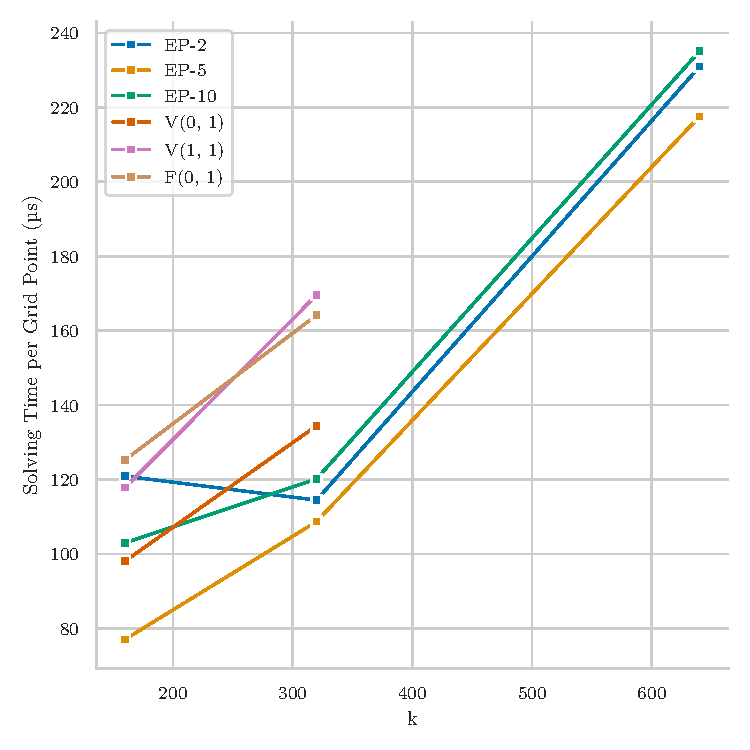
\includegraphics[width=\textwidth]{figures/solving-time.pdf}
	\caption{Solving time comparison of the best preconditioners according to the product of both objectives for different wavenumbers ($k$).}
	\label{fig:helmholtz-solving-time-comparison}
\end{figure} 
For better interpretability of the results, we have normalized each solving time by the number of grid points.
As the system of linear equations resulting from a discretization of Equation~\ref{eq:helmholtz-test-problem} becomes increasingly ill-conditioned for larger values of the wavenumber $k$, the relative cost to solve for each unknown grows accordingly.
All three discovered multigrid methods included in Figure~\ref{fig:helmholtz-solving-time-comparison} achieve a faster solving time than the best reference method V(0,1) while also staying competitive for smaller wavenumbers.
In particular, the overall best preconditioner EP-5 leads to a consistent improvement of 20 \% to the V(0,1) cycle.

Next, we need to address the question of why our evolutionary program synthesis did not consistently discover multigrid-based preconditioners that achieve the same degree of efficiency and generalizability in each experiment.
For this purpose, we again consider the space of non-dominated solutions at the end of each experiment, which is shown in Figure~\ref{fig:pareto-front-helmholtz}.
\begin{figure}
	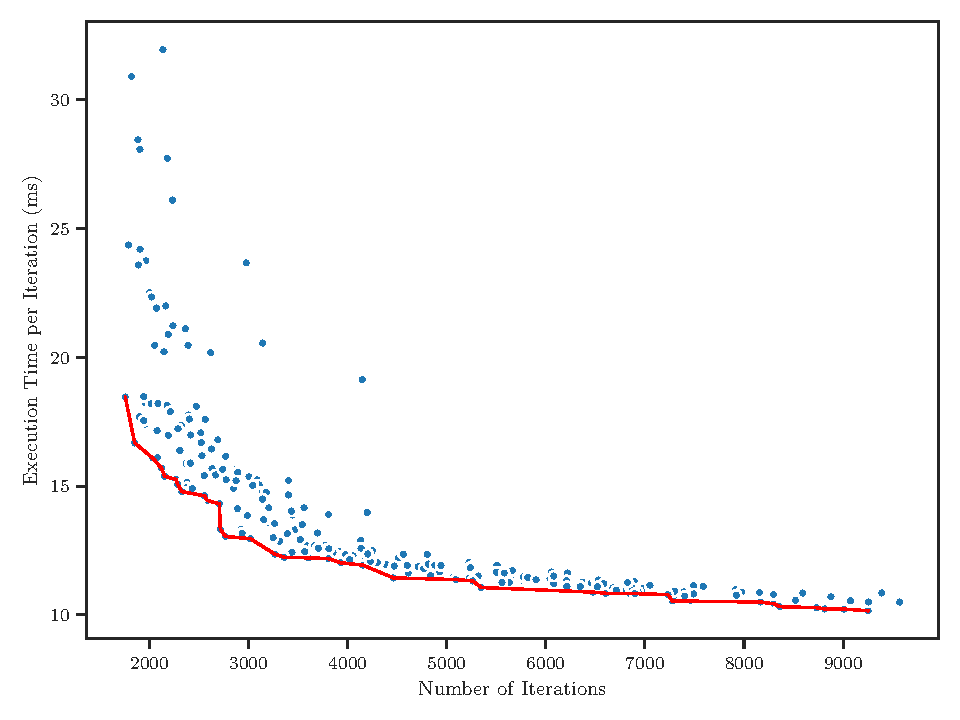
\includegraphics[width=\textwidth]{figures/pareto-front.pdf}
	\caption{Distribution of non-dominated solutions at the end of all ten experiments for $k = 320$. The red line denotes the combined front.}
	\label{fig:pareto-front-helmholtz}
\end{figure}
First of all, note that the number of non-dominated solutions is smaller than in the experiments performed in Section~\ref{sec:experiments-part1}.
However, this is clearly expected due to the smaller population size, which is only half as large as in our previous experiments.
Furthermore, as we iteratively increase the problem size and difficulty, the algorithm is forced to adapt the current population to the new characteristics of the problem within only 50 generations, which increases the difficulty of evolving the same number of non-dominated individuals. 
However, despite this fact, our evolutionary algorithm achieves a high degree of consistency in finding individuals that are located on the right half of the objective function space.
In contrast, in the left half of Figure~\ref{fig:pareto-front-helmholtz}, which corresponds to those individuals that lead to increasingly effective but more costly preconditioners, the algorithm is not able to find the same non-dominated individuals in each experiment.
Note that all multigrid-based preconditioners considered in our final evaluation shown in Table~\ref{table:evolved-solvers} correspond to individuals located here.
The larger distance of certain individuals in Figure~\ref{fig:pareto-front-helmholtz} to the combined front, therefore, explains why we could not achieve the same degree of efficiency in each run.
To reduce the number of iterations until convergence through preconditioning, we need to improve the accuracy of the approximate solution computed for Equation~\eqref{eq:helmholtz-test-problem-preconditioning}.
Since this requires us to perform more smoothing and coarse-grid correction steps, the size of the corresponding derivation trees grows accordingly.
In order to obtain the same derivation tree, we need to find an exact sequence of productions starting from a random initialization in each individual run of our algorithm.
As we have already investigated in Section~\ref{sec:experiments1-algorithm-behavior-analysis}, NSGA-II struggles to achieve this goal consistently~\cite{liu2022evolvability}, which, in certain experiments, leads to a suboptimal outcome in the leftmost part of the objective function space.

\subsection{Algorithmic Analysis}
While the results shown in Table~\ref{table:evolved-solvers} indicate that our automatically-designed preconditioners yield faster solvers than classical multigrid cycles for a wide range of different wavenumbers, we have not investigated how these methods are able to achieve this feat.
Therefore, we first need to gain an understanding of the computational structure of these methods and how it compares to those of classical multigrid cycles.
For this purpose, the Figures~\ref{fig:structure-evolved-preconditioners1} and ~\ref{fig:structure-evolved-preconditioners2} contain graphical representations of the six automatically-designed preconditioners EP-2, EP-3, EP4, EP-5, EP-8 and EP-10 that yield a converging solver for a wavenumber of $k = 640$, for which all classical multigrid cycles fail to achieve convergence.
\begin{figure}
\captionsetup[subfigure]{justification=centering}
\begin{subfigure}[b]{\columnwidth}
		\scalebox{0.75}{%
			\begin{tikzpicture}
			\node   (h) at (-0.75, 4){$h$};
			\node   (2h) at (-0.75, 3){$2h$};
			\node   (4h) at (-0.75, 2){$4h$};
			\node   (8h) at (-0.75, 1){$8h$};
			\node   (16h) at (-0.75, 0){$16h$};
			\node	(a) at (0,4) [draw, circle,inner sep=0pt,minimum size=5mm] {\phantom{\tiny 1.00}};
			\node	(b) at (0.5,3) [draw, circle,inner sep=0pt,minimum size=5mm] {\phantom{\tiny 1.00}};
			\node	(c) at (1,2) [draw, circle,fill=lightred,inner sep=0pt,minimum size=5mm] {\tiny 1.00};
			\node	(d) at (1.5,1) [draw, circle,inner sep=0pt,minimum size=5mm] {\phantom{\tiny 1.00}};
			\node	(e) at (2,0) [draw, circle,fill=black, inner sep=0pt,minimum size=5mm] {\phantom{\tiny 1.00}};
			\node	(f) at (2.5,1) [draw, circle,inner sep=0pt,minimum size=5mm] {\phantom{\tiny 1.00}};
			\node	(g) at (3,2) [draw, circle,inner sep=0pt,minimum size=5mm] {\phantom{\tiny 1.00}};
			\node	(h) at (3.5,3) [draw, circle,fill=lightred,inner sep=0pt,minimum size=5mm] {\tiny 0.90};
			\node	(i) at (4.5,3) [draw, circle,fill=lightred,inner sep=0pt,minimum size=5mm] {\tiny 1.20};
			\node	(j) at (5,2) [draw, circle,fill=lightred, inner sep=0pt,minimum size=5mm] {\tiny 1.40};
			\node	(k) at (5.5,1) [draw, circle,fill=lightblue,inner sep=0pt,minimum size=5mm] {\tiny 1.00};
			\node	(l) at (6,2) [draw, circle,inner sep=0pt,minimum size=5mm] {\phantom{\tiny 1.00}};
			\node	(m) at (6.5,3) [draw, circle, fill=lightred, inner sep=0pt,minimum size=5mm] {\tiny 1.20};
			\node	(n) at (7,2) [draw, circle,fill=lightred, inner sep=0pt,minimum size=5mm] {\tiny 1.40};
			\node	(o) at (7.5,1) [draw, circle, fill=lightred, inner sep=0pt,minimum size=5mm] {\tiny 0.65};
			\node	(p) at (8,2) [draw, circle, inner sep=0pt,minimum size=5mm] {\phantom{\tiny 1.00}};
			\node	(q) at (8.5,3) [draw, circle, fill=lightred, inner sep=0pt,minimum size=5mm] {\tiny 1.20};
			\node	(r) at (9,2) [draw, circle, fill=lightred, inner sep=0pt,minimum size=5mm] {\tiny 1.25};
			\node	(s) at (9.5,1) [draw, circle, fill=lightred, inner sep=0pt,minimum size=5mm] {\tiny 1.45};
			\node	(t) at (10,2) [draw, circle, inner sep=0pt,minimum size=5mm] {\phantom{\tiny 1.00}};
			\node	(u) at (10.5,3) [draw, circle, fill=lightred, inner sep=0pt,minimum size=5mm] {\tiny 1.10};
			\node	(v) at (11,4) [draw, circle, fill=lightred, inner sep=0pt,minimum size=5mm] {\tiny 0.80};
			%\node	(w) at (11,4) [draw, circle, fill=lightred, inner sep=0pt,minimum size=5mm] {};
			\draw 
			(a) edge[->] (b) 
			(b) edge[->] (c)
			(c) edge[->] (d)
			(d) edge[->] (e)   
			(e) edge[->] node[near end,left] {\tiny 1.00} (f)
			(f) edge[->] node[near end,left] {\tiny 1.60} (g)
			(g) edge[->] node[near end,left] {\tiny 0.85} (h)
			(h) edge[->] (i)
			(i) edge[->] (j) 
			(j) edge[->] (k)
			(k) edge[->] node[near end,left] {\tiny 0.30} (l)
			(l) edge[->] node[near end,left] {\tiny 0.85} (m)   
			(m) edge[->] (n)
			(n) edge[->] (o)
			(o) edge[->] node[near end,left] {\tiny 0.30} (p)
			(p) edge[->] node[near end,left] {\tiny 0.85} (q)
			(q) edge[->] (r)
			(r) edge[->] (s)
			(s) edge[->] node[near end,left] {\tiny 0.30} (t)
			(t) edge[->] node[near end,left] {\tiny 0.85} (u)
			(u) edge[->] node[near end,left] {\tiny 1.35} (v)
			%(v) edge[->] (w)
			;
			\end{tikzpicture}
		}
		\caption{EP-2}
		\label{fig:ep-2}
	\end{subfigure}
  \par\bigskip
	\begin{subfigure}[b]{0.465\columnwidth}
		\scalebox{0.75}{%
			\begin{tikzpicture}
			\node   (h) at (-0.75, 4){$h$};
			\node   (2h) at (-0.75, 3){$2h$};
			\node   (4h) at (-0.75, 2){$4h$};
			\node   (8h) at (-0.75, 1){$8h$};
			\node   (16h) at (-0.75, 0){$16h$};
			\node	(a) at (0,4) [draw, circle,inner sep=0pt,minimum size=5mm] {\phantom{\tiny 1.00}};
			\node	(b) at (0.5,3) [draw, circle,inner sep=0pt,minimum size=5mm] {\phantom{\tiny 1.00}};
			\node	(c) at (1,2) [draw, circle,fill=lightblue,inner sep=0pt,minimum size=5mm] {\tiny 1.25};
			\node	(d) at (1.5,1) [draw, circle,inner sep=0pt,minimum size=5mm] {\phantom{\tiny 1.00}};
			\node	(e) at (2,0) [draw, circle,fill=black, inner sep=0pt,minimum size=5mm] {\phantom{\tiny 1.00}};
			\node	(f) at (2.5,1) [draw, circle,fill=lightred,inner sep=0pt,minimum size=5mm] {\tiny 1.05};
			\node	(g) at (3,2) [draw, circle,inner sep=0pt,minimum size=5mm] {\phantom{\tiny 1.00}};
			\node	(h) at (3.5,3) [draw, circle,fill=lightred,inner sep=0pt,minimum size=5mm] {\tiny 1.25};
			\node	(i) at (4,2) [draw, circle,fill=lightred,inner sep=0pt,minimum size=5mm] {\tiny 1.15};
			\node	(j) at (4.5,3) [draw, circle,fill=lightred, inner sep=0pt,minimum size=5mm] {\tiny 1.25};
			\node	(k) at (5,2) [draw, circle,fill=lightred,inner sep=0pt,minimum size=5mm] {\tiny 1.10};
			\node	(l) at (5.5,3) [draw, circle, fill=lightred, inner sep=0pt,minimum size=5mm] {\tiny 1.25};
			\node	(m) at (6,4) [draw, circle,fill=lightred, inner sep=0pt,minimum size=5mm] {\tiny 0.75};
			%\node	(w) at (11,4) [draw, circle, fill=lightred, inner sep=0pt,minimum size=5mm] {};
			\draw 
			(a) edge[->] (b) 
			(b) edge[->] (c)
			(c) edge[->] (d)
			(d) edge[->] (e)   
			(e) edge[->] node[near end,left] {\tiny 1.00} (f)
			(f) edge[->] node[near end,left] {\tiny 1.25} (g)
			(g) edge[->] node[near end,left] {\tiny 1.05} (h)
			(h) edge[->] (i)
			(i) edge[->] node[near end,left] {\tiny 0.90} (j) 
			(j) edge[->] (k)
			(k) edge[->] node[near end,left] {\tiny 0.90} (l)
			(l) edge[->] node[near end,left] {\tiny 1.40} (m)   
			;
			\end{tikzpicture}
		}
		\caption{EP-3}
		\label{fig:ep-3}
	\end{subfigure}
     \begin{subfigure}[b]{0.5\columnwidth}
		\scalebox{0.75}{%
			\begin{tikzpicture}
			\node	(a) at (0,4) [draw, circle,inner sep=0pt,minimum size=5mm] {\phantom{\tiny 1.00}};
			\node	(b) at (0.5,3) [draw, circle,fill=lightred,inner sep=0pt,minimum size=5mm] {\tiny 1.15};
			\node	(c) at (1,2) [draw,circle,fill=lightblue, inner sep=0pt,minimum size=5mm] {\tiny 1.55};
			\node	(d) at (1.5,1) [draw,circle,fill=lightred, inner sep=0pt,minimum size=5mm] {\tiny 1.05};
			\node	(e) at (2,0) [draw, circle,fill=black, inner sep=0pt,minimum size=5mm] {\phantom{\tiny 1.00}};
			\node	(f) at (2.5,1) [draw, circle, inner sep=0pt,minimum size=5mm] {\phantom{\tiny 1.00}};
			\node	(g) at (3,2) [draw, circle, inner sep=0pt,minimum size=5mm] {\phantom{\tiny 1.00}};
			\node	(h) at (3.5,3) [draw, circle,fill=lightred, inner sep=0pt,minimum size=5mm] {\tiny 1.00};
			\node	(i) at (4,2) [draw, circle,fill=lightred, inner sep=0pt,minimum size=5mm] {\tiny 0.95};
			\node	(j) at (4.5,3) [draw, circle, inner sep=0pt,minimum size=5mm] {\phantom{\tiny 1.00}};
			\node	(k) at (5,2) [draw, circle,fill=lightred, inner sep=0pt,minimum size=5mm] {\tiny 0.70};
			\node	(l) at (5.5,3) [draw, circle, inner sep=0pt,minimum size=5mm] {\phantom{\tiny 1.00}};
			\node	(m) at (6,4) [draw, circle,fill=lightred, inner sep=0pt,minimum size=5mm] {\tiny 1.00};
			\node	(n) at (6.5,3) [draw, circle, inner sep=0pt,minimum size=5mm] {\phantom{\tiny 1.00}};
			\node	(o) at (7,2) [draw, circle, fill=lightred,inner sep=0pt,minimum size=5mm] {\tiny 0.70};
			\node	(p) at (7.5,3) [draw, circle, inner sep=0pt,minimum size=5mm] {\phantom{\tiny 1.00}};
			\node	(q) at (8,4) [draw, circle, inner sep=0pt,minimum size=5mm] {\phantom{\tiny 1.00}};
			\draw 
			(a) edge[->] (b) 
			(b) edge[->] (c)
			(c) edge[->] (d)
			(d) edge[->] (e)   
			(e) edge[->] node[near end,left] {\tiny 1.00}  (f)
			(f) edge[->] node[near end,left] {\tiny 0.95} (g)
			(g) edge[->] node[near end,left] {\tiny 1.45} (h)
			(h) edge[->] (i)
			(i) edge[->] node[near end,left] {\tiny 1.30} (j) 
			(j) edge[->] (k)
			(k) edge[->] node[near end,left] {\tiny 1.10} (l)
			(l) edge[->] node[near end,left] {\tiny 1.65} (m)   
			(m) edge[->] (n)
			(n) edge[->] (o)
			(o) edge[->] node[near end,left] {\tiny 1.10} (p)
			(p) edge[->] node[near end,left] {\tiny 1.20} (q)
			;
			\end{tikzpicture}
		}
		\caption{EP-8}
		\label{fig:ep-8}
	\end{subfigure}
    \par\bigskip
  	\begin{subfigure}[b]{\columnwidth}
			\scalebox{0.75}{%
			\begin{tikzpicture}
			\node   (h) at (-0.75, 4){$h$};
			\node   (2h) at (-0.75, 3){$2h$};
			\node   (4h) at (-0.75, 2){$4h$};
			\node   (8h) at (-0.75, 1){$8h$};
			\node   (16h) at (-0.75, 0){$16h$};
			\node	(a) at (0,4) [draw, circle,inner sep=0pt,minimum size=5mm] {\phantom{\tiny 1.00}};
			\node	(b) at (0.5,3) [draw, circle,fill=lightred,inner sep=0pt,minimum size=5mm] {\tiny 1.10};
			\node	(c) at (1.5,3) [draw, circle,fill=lightblue,inner sep=0pt,minimum size=5mm] {\tiny 0.95};
			\node	(d) at (2,2) [draw, circle,inner sep=0pt,minimum size=5mm] {\phantom{\tiny 1.00}};
			\node	(e) at (2.5,1) [draw, circle,fill=lightblue,inner sep=0pt,minimum size=5mm] {\tiny 1.05};
			\node	(f) at (3,0) [draw, fill=black,circle,inner sep=0pt,minimum size=5mm] {\phantom{\tiny 1.00}};
			\node	(g) at (3.5,1) [draw, circle,inner sep=0pt,minimum size=5mm] {\phantom{\tiny 1.00}};
			\node	(h) at (4,2) [draw, circle,fill=lightred,inner sep=0pt,minimum size=5mm] {\tiny 1.70};
			\node	(i) at (4.5,1) [draw, circle,inner sep=0pt,minimum size=5mm] {\phantom{\tiny 1.00}};
			\node	(j) at (5,0) [draw, circle,fill=black,inner sep=0pt,minimum size=5mm] {\phantom{\tiny 1.00}};
			\node	(k) at (5.5,1) [draw, circle,inner sep=0pt,minimum size=5mm] {\phantom{\tiny 1.00}};
			\node	(l) at (6,2) [draw, circle,fill=lightblue,inner sep=0pt,minimum size=5mm] {\tiny 0.30};
			\node	(m) at (6.5,3) [draw, circle, inner sep=0pt,minimum size=5mm] {\phantom{\tiny 1.00}};
			\node	(n) at (7,2) [draw, circle,fill=lightred, inner sep=0pt,minimum size=5mm] {\tiny 0.45};
			\node	(o) at (7.5,3) [draw, circle, inner sep=0pt,minimum size=5mm] {\phantom{\tiny 1.00}};
			\node	(p) at (8,4) [draw, circle, inner sep=0pt,minimum size=5mm] {\phantom{\tiny 1.00}};
			\node	(q) at (8.5,3) [draw, circle, inner sep=0pt,minimum size=5mm] {\phantom{\tiny 1.00}};
			\node	(r) at (9,2) [draw, circle, fill=lightblue, inner sep=0pt,minimum size=5mm] {\tiny 1.70};
			\node	(s) at (9.5,3) [draw, circle, inner sep=0pt,minimum size=5mm] {\phantom{\tiny 1.00}};
			\node	(t) at (10,4) [draw, circle, inner sep=0pt,minimum size=5mm] {\phantom{\tiny 1.00}};
			\node	(u) at (10.5,3) [draw, circle, inner sep=0pt,minimum size=5mm] {\phantom{\tiny 1.00}};
			\node	(v) at (11,2) [draw, circle, fill=lightblue, inner sep=0pt,minimum size=5mm] {\tiny 1.05};
			\node	(w) at (11.5,3) [draw, circle, inner sep=0pt,minimum size=5mm] {\phantom{\tiny 1.00}};
   			\node	(x) at (12,4) [draw, circle, inner sep=0pt,minimum size=5mm] {\phantom{\tiny 1.00}};
      		\node	(y) at (12.5,3) [draw, circle, inner sep=0pt,minimum size=5mm] {\phantom{\tiny 1.00}};
			\node	(z) at (13,2) [draw, circle, fill=lightblue, inner sep=0pt,minimum size=5mm] {\tiny 0.30};
			\node	(aa) at (13.5,3) [draw, circle, inner sep=0pt,minimum size=5mm] {\phantom{\tiny 1.00}};
   			\node	(bb) at (14,4) [draw, circle, inner sep=0pt,minimum size=5mm] {\phantom{\tiny 1.00}};
            \node	(cc) at (14.5,3) [draw, circle, fill=lightblue, inner sep=0pt,minimum size=5mm] {\tiny 1.25};
   			\node	(dd) at (15,4) [draw, circle, fill=lightred, inner sep=0pt,minimum size=5mm] {\tiny 1.05};
			\draw 
			(a) edge[->] (b) 
			(b) edge[->] (c)
			(c) edge[->] (d)
			(d) edge[->] (e)   
			(e) edge[->] (f)
			(f) edge[->] node[near end,left] {\tiny 1.00} (g)
			(g) edge[->] node[near end,left] {\tiny 0.80} (h)
			(h) edge[->] (i)
			(i) edge[->] (j) 
			(j) edge[->] node[near end,left] {\tiny 1.00} (k)
			(k) edge[->] node[near end,left] {\tiny 0.55} (l)
			(l) edge[->] node[near end,left] {\tiny 1.70} (m)   
			(m) edge[->] (n)
			(n) edge[->] node[near end,left] {\tiny 1.80} (o)
			(o) edge[->] node[near end,left] {\tiny 1.70} (p)
			(p) edge[->] (q)
			(q) edge[->] (r)
			(r) edge[->] node[near end,left] {\tiny 0.95} (s)
			(s) edge[->] node[near end,left] {\tiny 1.10} (t)
			(t) edge[->] (u)
			(u) edge[->] (v)
			(v) edge[->] node[near end,left] {\tiny 0.55} (w)
   			(w) edge[->] node[near end,left] {\tiny 0.95} (x)
      		(x) edge[->] (y)
			(y) edge[->] (z)
			(z) edge[->] node[near end,left] {\tiny 0.95} (aa)
   			(aa) edge[->] node[near end,left] {\tiny 1.10} (bb)
      		(bb) edge[->] (cc)
   			(cc) edge[->] node[near end,left] {\tiny 0.90} (dd)
			;
			\end{tikzpicture}
		}
		\caption{EP-4}
		\label{fig:ep-4}
	\end{subfigure}
	\caption{Computational structure of the evolved multigrid preconditioners EP-2, EP-3, EP-8 and EP-4. The color of the node denotes the type of operation. Black: Coarse-grid solver, Blue: Pointwise Jacobi smoothing, Red: Red-black Gauss-Seidel smoothing, White: No operation. The relaxation factor of each smoothing step is included in each node, while for coarse-grid correction, it is attached to the respective edge.}
	\label{fig:structure-evolved-preconditioners1}
\end{figure}
\begin{figure}
\captionsetup[subfigure]{justification=centering}
	\begin{subfigure}[b]{\columnwidth}
		\scalebox{0.75}{%
			\begin{tikzpicture}
			\node   (h) at (-0.75, 4){$h$};
			\node   (2h) at (-0.75, 3){$2h$};
			\node   (4h) at (-0.75, 2){$4h$};
			\node   (8h) at (-0.75, 1){$8h$};
			\node   (16h) at (-0.75, 0){$16h$};
			\node	(a) at (0,4) [draw, circle,inner sep=0pt,minimum size=5mm] {\phantom{\tiny 1.00}};
			\node	(b) at (0.5,3) [draw, circle,fill=lightred,inner sep=0pt,minimum size=5mm] {\tiny 1.30};
			\node	(c) at (1,2) [draw,circle,fill=lightblue, inner sep=0pt,minimum size=5mm] {\tiny 1.45};
			\node	(d) at (1.5,1) [draw,circle,fill=lightblue, inner sep=0pt,minimum size=5mm] {\tiny 1.35};
			\node	(e) at (2,0) [draw, circle,fill=black, inner sep=0pt,minimum size=5mm] {\phantom{\tiny 1.00}};
			\node	(f) at (2.5,1) [draw, circle, inner sep=0pt,minimum size=5mm] {\phantom{\tiny 1.00}};
			\node	(g) at (3,2) [draw, circle, inner sep=0pt,minimum size=5mm] {\phantom{\tiny 1.00}};
			\node	(h) at (3.5,3) [draw, circle, inner sep=0pt,minimum size=5mm] {\phantom{\tiny 1.00}};
			\node	(i) at (4,4) [draw, circle,fill=lightred, inner sep=0pt,minimum size=5mm] {\tiny 1.20};
			\node	(j) at (4.5,3) [draw, circle, inner sep=0pt,minimum size=5mm] {\phantom{\tiny 1.00}};
			\node	(k) at (5,2) [draw, circle,fill=lightred, inner sep=0pt,minimum size=5mm] {\tiny 1.30};
			\node	(l) at (5.5,3) [draw, circle, inner sep=0pt,minimum size=5mm] {\phantom{\tiny 1.00}};
			\node	(m) at (6,2) [draw, circle,fill=lightblue, inner sep=0pt,minimum size=5mm] {\tiny 1.80};
			\node	(n) at (7,2) [draw, circle,fill=lightblue, inner sep=0pt,minimum size=5mm] {\tiny 0.55};
			\node	(o) at (7.5,3) [draw, circle, inner sep=0pt,minimum size=5mm] {\phantom{\tiny 1.00}};
			\node	(p) at (8,2) [draw, circle, fill=lightred, inner sep=0pt,minimum size=5mm] {\tiny 1.80};
			\node	(q) at (8.5,1) [draw, circle, fill=lightred, inner sep=0pt,minimum size=5mm] {\tiny 1.45};
			\node	(r) at (9,2) [draw, circle, inner sep=0pt,minimum size=5mm] {\phantom{\tiny 1.00}};
			\node	(s) at (9.5,3) [draw, circle, inner sep=0pt,minimum size=5mm] {\phantom{\tiny 1.00}};
			\node	(t) at (10,2) [draw, circle, fill=lightblue, inner sep=0pt,minimum size=5mm] {\tiny 0.95};
			\node	(u) at (11,2) [draw, circle, fill=lightred, inner sep=0pt,minimum size=5mm] {\tiny 0.70};
			\node	(v) at (11.5,3) [draw, circle, fill=lightred, inner sep=0pt,minimum size=5mm] {\tiny 1.00};
			\node	(w) at (12,4) [draw, circle, fill=lightred, inner sep=0pt,minimum size=5mm] {\tiny 0.90};
			\draw 
			(a) edge[->] (b) 
			(b) edge[->] (c)
			(c) edge[->] (d)
			(d) edge[->] (e)   
			(e) edge[->] node[near end,left] {\tiny 1.00}  (f)
			(f) edge[->] node[near end,left] {\tiny 1.00} (g)
			(g) edge[->] node[near end,left] {\tiny 0.80} (h)
			(h) edge[->] node[near end,left] {\tiny 1.60} (i)
			(i) edge[->] (j) 
			(j) edge[->] (k)
			(k) edge[->] node[near end,left] {\tiny 0.85} (l)
			(l) edge[->] (m)   
			(m) edge[->] (n)
			(n) edge[->] node[near end,left] {\tiny 0.85} (o)
			(o) edge[->] (p)
			(p) edge[->] (q)
			(q) edge[->] node[near end,left] {\tiny 1.05} (r)
			(r) edge[->] node[near end,left] {\tiny 1.10} (s)
			(s) edge[->] (t)
			(t) edge[->] (u)
			(u) edge[->] node[near end,left] {\tiny 1.05} (v)
			(v) edge[->] node[near end,left] {\tiny 1.80} (w)
			;
			\end{tikzpicture}
		}
		\caption{EP-5}
		\label{fig:ep-5}
	\end{subfigure}
  \par\bigskip
 	\begin{subfigure}[b]{\columnwidth}
			\scalebox{0.75}{%
			\begin{tikzpicture}
			\node   (h) at (-0.75, 4){$h$};
			\node   (2h) at (-0.75, 3){$2h$};
			\node   (4h) at (-0.75, 2){$4h$};
			\node   (8h) at (-0.75, 1){$8h$};
			\node   (16h) at (-0.75, 0){$16h$};
			\node	(a) at (0,4) [draw, circle,inner sep=0pt,minimum size=5mm] {\phantom{\tiny 1.00}};
			\node	(b) at (0.5,3) [draw, circle,inner sep=0pt,minimum size=5mm] {\phantom{\tiny 1.00}};
			\node	(c) at (1,2) [draw, circle,inner sep=0pt,minimum size=5mm] {\phantom{\tiny 1.00}};
			\node	(d) at (1.5,1) [draw, circle,inner sep=0pt,minimum size=5mm] {\phantom{\tiny 1.00}};
			\node	(e) at (2,0) [draw, circle,fill=black, inner sep=0pt,minimum size=5mm] {\phantom{\tiny 1.00}};
			\node	(f) at (2.5,1) [draw, circle,inner sep=0pt,minimum size=5mm] {\phantom{\tiny 1.00}};
			\node	(g) at (3,2) [draw, circle,fill=lightred,inner sep=0pt,minimum size=5mm] {\tiny 0.55};
			\node	(h) at (3.5,3) [draw, circle,fill=lightred,inner sep=0pt,minimum size=5mm] {\tiny 1.40};
			\node	(i) at (4,2) [draw, circle,fill=lightred,inner sep=0pt,minimum size=5mm] {\tiny 1.15};
			\node	(j) at (4.5,3) [draw, circle,fill=lightred, inner sep=0pt,minimum size=5mm] {\tiny 1.10};
			\node	(k) at (5,2) [draw, circle,fill=lightblue,inner sep=0pt,minimum size=5mm] {\tiny 1.50};
			\node	(l) at (6,2) [draw, circle,fill=lightred,inner sep=0pt,minimum size=5mm] {\tiny 0.20};
			\node	(m) at (7,2) [draw, circle, fill=lightred, inner sep=0pt,minimum size=5mm] {\tiny 0.55};
			\node	(n) at (7.5,3) [draw, circle,fill=lightred, inner sep=0pt,minimum size=5mm] {\tiny 1.40};
			\node	(o) at (8,2) [draw, circle, fill=lightred, inner sep=0pt,minimum size=5mm] {\tiny 0.65};
			\node	(p) at (8.5,3) [draw, circle,fill=lightred, inner sep=0pt,minimum size=5mm] {\tiny 1.10};
			\node	(q) at (9,2) [draw, circle, fill=lightblue, inner sep=0pt,minimum size=5mm] {\tiny 0.25};
			\node	(r) at (10,2) [draw, circle, fill=lightred, inner sep=0pt,minimum size=5mm] {\tiny 1.05};
			\node	(s) at (10.5,3) [draw, circle, inner sep=0pt,minimum size=5mm] {\phantom{\tiny 1.00}};
			\node	(t) at (11,4) [draw, circle, inner sep=0pt,minimum size=5mm] {\phantom{\tiny 1.00}};
			\node	(u) at (11.5,3) [draw, circle, inner sep=0pt,minimum size=5mm] {\phantom{\tiny 1.00}};
			\node	(v) at (12,2) [draw, circle, fill=lightred, inner sep=0pt,minimum size=5mm] {\tiny 0.65};
			\node	(w) at (12.5,3) [draw, circle, fill=lightred, inner sep=0pt,minimum size=5mm] {\tiny 1.25};
   			\node	(x) at (13,4) [draw, circle, fill=lightred, inner sep=0pt,minimum size=5mm] {\tiny 0.80};
			\draw 
			(a) edge[->] (b) 
			(b) edge[->] (c)
			(c) edge[->] (d)
			(d) edge[->] (e)   
			(e) edge[->] node[near end,left] {\tiny 1.00} (f)
			(f) edge[->] node[near end,left] {\tiny 0.70} (g)
			(g) edge[->] node[near end,left] {\tiny 1.10} (h)
			(h) edge[->] (i)
			(i) edge[->] node[near end,left] {\tiny 0.85} (j) 
			(j) edge[->] (k)
			(k) edge[->] (l)
			(l) edge[->] (m)   
			(m) edge[->] node[near end,left] {\tiny 1.00} (n)
			(n) edge[->] (o)
			(o) edge[->] node[near end,left] {\tiny 1.40} (p)
			(p) edge[->] (q)
			(q) edge[->] (r)
			(r) edge[->] node[near end,left] {\tiny 1.70} (s)
			(s) edge[->] node[near end,left] {\tiny 1.65} (t)
			(t) edge[->] (u)
			(u) edge[->] (v)
			(v) edge[->] node[near end,left] {\tiny 1.40} (w)
   			(w) edge[->] node[near end,left] {\tiny 0.80} (x)
			;
			\end{tikzpicture}
		}
		\caption{EP-10}
		\label{fig:ep-10}
	\end{subfigure}
	\caption{Computational structure of the evolved multigrid preconditioners EP-5 and EP-10. The color of the node denotes the type of operation. Black: Coarse-grid solver, Blue: Pointwise Jacobi smoothing, Red: Red-black Gauss-Seidel smoothing, White: No operation. The relaxation factor of each smoothing step is included in each node, while for coarse-grid correction, it is attached to the respective edge.}
	\label{fig:structure-evolved-preconditioners2}
\end{figure}
As illustrated by their graphical representations, the employed sequence of multigrid operations varies wildly between the individual methods, and none of them can easily be characterized as one of the classical multigrid cycles.
However, we can still identify a number of common characteristics.
First of all, while we have also included different block Jacobi smoothers into the search space, each of our automatically-designed methods employs exclusively pointwise Jacobi and red-black Gauss-Seidel smoothing, whereby, with the exception of EP-3, the latter is used predominantly.
If we consider the total amount of smoothing used within each method, we can deduce that, on average, Jacobi is used in $1/3$ of the smoothing steps.
However, in contrast to classical multigrid cycles, both the type of smoother and relaxation factor can be varied in each step, which stems from the capability of our evolutionary program synthesis method to alter each computational step within the sequence without affecting the rest.
If we examine the computational structure of the methods more closely, we can see that many coarse-grid correction steps originate from one or multiple smoothing steps on intermediate levels, often using a different combination of relaxation factors.
In contrast, again, with the exception of EP-4, each method only employs the coarse-grid solver only once, which is then proceeded with multiple smoothing-based coarse-grid corrections on intermediate levels, whereby often individual smoothing steps are completely skipped.
If we consider that EP-5 represents the overall most efficient preconditioner for different wavenumbers, we can see that here, a combination of different smoothers and relaxation factors within these correction steps seems to be the most effective approach.
Furthermore, note that in contrast to classical multigrid methods, the number of smoothing and coarse-grid correction steps is unevenly distributed over the range of levels.
Table~\ref{table:operations-per-level} shows the average number of smoothing steps, coarse-grid correction steps, and the number of updates of the approximate solution\footnote{Note that this includes both smoothing and coarse-grid correction steps} on every level.
As this analysis reveals, the number of operations on the intermediate levels $2h$ and $4h$ is significantly higher than on the higher and lower levels, which means that these levels seem to be most cost-effective for accelerating the convergence of the BiCGSTAB solver.
Here it is especially interesting that instead of applying the combined error reduction of all smoothing steps in a single coarse-grid correction, as it is usually performed in classical multigrid cycles, the correction is split into multiple steps, such that, on average, the total number of coarse-grid corrections is roughly equal to the number of smoothing steps.
To gain a better understanding of the consequences of this strategy, consider the method EP-3, which uses the lowest total number of operations, and, thus, leads to the highest number of iterations.
If we compare the solving time and the number of iterations this method achieves according to Table~\ref{table:evolved-solvers}, with the characteristics of the classical multigrid cycles shown in Table~\ref{table:reference-methods-helmholtz}, we can see that it converges as fast as the W(3,3)-cycle while requiring 69 - 75 \% less time per iteration.
While especially EP-2, EP-5 and EP-10 utilize a higher number of coarse-grid corrections and smoothing steps to achieve faster convergence, the simplicity of the EP-3 method demonstrates that the alternation of smoothers and relaxation factors combined with the addition of only two smoothing-based correction steps on intermediate levels can yield a remarkably efficient preconditioner for the indefinite Helmholtz equation.
The EP-4 represents another noteworthy exception. 
In contrast to the other multigrid-based preconditions, which more closely resemble V-cycles, as they all apply the coarse-grid solver only once, this method combines a four-grid W-cycle with a series of smoothing-based coarse-grid corrections, each of which is structurally similar to a three-grid V-cycle whereby the coarse-grid solver is replaced by a single Jacobi-step.
In general, the distinct sequences of operations shown in Figure~\ref{fig:structure-evolved-preconditioners1} and~\ref{fig:structure-evolved-preconditioners2} demonstrate that our evolutionary program synthesis approach is capable of discovering multigrid methods with novel algorithmic strategies that have not yet been investigated in the literature.
Since the utilization of different relaxation factors within each smoothing and coarse-grid correction step represents an integral feature of all six investigated multigrid-based preconditioners, as the last step within this analysis, we investigate their overall distribution of relaxation factors.
For this purpose, Figure~\ref{fig:histograms} contains a histogram of the distribution of relaxation factors used within each red-black Gauss-Seidel and coarse-grid correction step, respectively.
Since the number of Jacobi steps is significantly smaller and, thus, does not permit a reliable statistical analysis, the corresponding histogram is omitted here.



% First of all, both multigrid methods employ a unique sequence of operations that does not resemble any known multigrid cycle.
% While both methods initially apply the coarse-grid solver exactly once and, thus, resemble a V-cycle, they incorporate additional smoothing-based coarse-grid correction steps.
% Furthermore, our grammar-based representation enables the combination of different smoothers or even the complete omission of smoothing on certain levels.
% While both methods employ predominantly red-black Gauss-Seidel smoothing, especially EP-2 also incorporates multiple intermediate Jacobi steps.
% With respect to the number of smoothing steps, similar to the most efficient reference methods, V(0,1), V(1,1), and F(0,1), smoothing on the finest grid is reduced to a bare minimum, in the form of one or two red-black Gauss-Seidel steps.
% However, this is augmented with a significantly larger number of smoothing and coarse-grid correction steps on subsequent levels, which is in contrast to the uniform structure of classical multigrid cycles.
% In general, the computational structure of EP-2 comprises a higher degree of regularity since, at its end,
% the same sequence of operations is repeated three times.
% While within each execution of this sequence, the relaxation factors of certain smoothing operations are altered, the same two values, 0.30 and 0.85, are employed within the two coarse-grid correction steps.
% The computational structure of EP-5 is less uniform compared to EP-2.
% However, on the second finest grid, the method repeatedly applies a similar sequence of restriction, smoothing, and prolongation, whereby in each step, a different combination of smoothers is used.
% The resulting effectiveness of both multigrid methods as a preconditioner, together with their high computational efficiency, highlights the advantages of our grammar-based representation.
% The construction of both methods requires the alternation of individual operations within their sequence.
% Encoding the computational structure of a multigrid method based on a number of global parameters does not come with that flexibility.
% For instance, choosing a different value for $\mu$ in Algorithm~\ref{alg:multigrid-cycle} changes the number of recursive descents on each level of the method.
% However, none of the available parameters offers a way to insert a single coarse-grid correction or smoothing step after at a specific position within the sequence.
% In contrast, expressing each computational step in the form of a separate production within a formal grammar allows us to achieve this goal by inserting the corresponding subtree into the respective derivation tree, as discussed in Section~\ref{sec:gggp} and Chapter~\ref{chapter:multigrid-formal-language}.
\begin{table}
	\caption{Statistics about the operations that are performed by the preconditioners that yield a converging solver for $k = 640$ on every level.}
	\label{table:operations-per-level}
	\centering
	\begin{tabular}{l c c c c c c c}
		\toprule
  		& \multicolumn{3}{c}{Smoothing} & \multicolumn{3}{c}{Coarse-Grid Correction} & \\
		\cmidrule(l){2-4} \cmidrule(l){5-7}
		Level & Mean & Min & Max & Mean & Min & Max & Mean Updates \\
        \midrule
        $h$ & $1.17$ & $1$ & $2$ & $2.17$ & $1$ & $5$ & $3.33$\\
        \midrule
        $2h$ & $3.33$ & $2$ & $5$ & $4.50$ & $3$ & $6$ & $7.83$ \\
        \midrule
        $4h$ & $5.50$ & $3$ & $9$ & $1.83$ & $1$ & $4$ & $7.33$ \\
        \midrule
        $8h$ & $1.33$ & $0$ & $3$ & $1.17$ & $1$ & $2$ & $2.50$ \\
		\bottomrule
	\end{tabular}
\end{table}
\begin{figure}
\captionsetup[subfigure]{justification=centering}
\begin{subfigure}[b]{\textwidth}
	\centering
    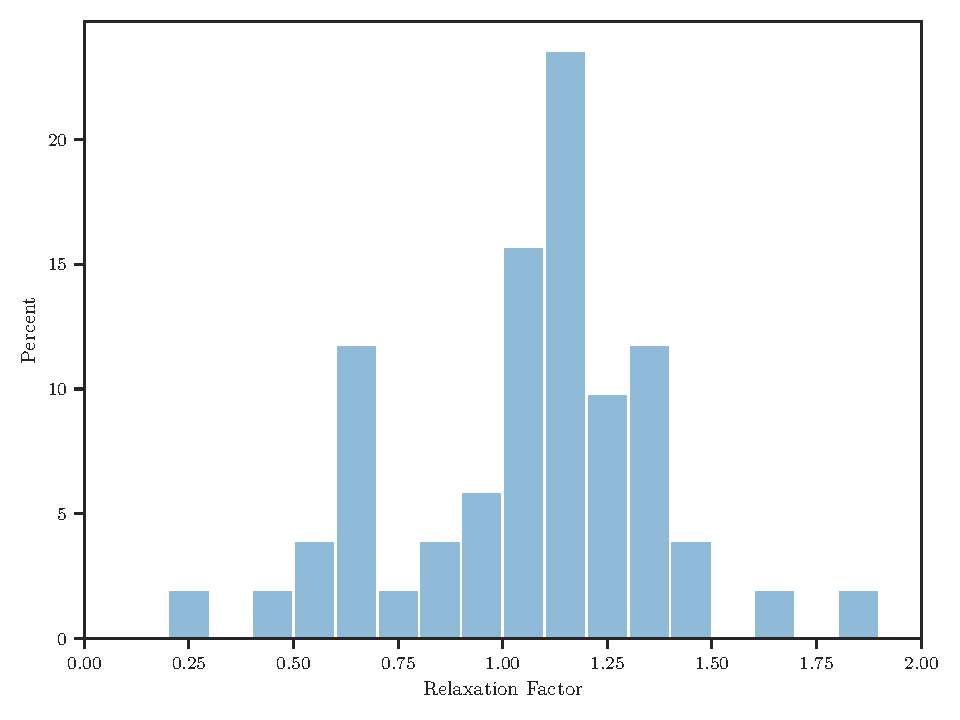
\includegraphics[height=0.4\textheight]{figures/histogram_rbgs.pdf}
	\caption{Red-black Gauss-Seidel}
	\label{fig:histogram-rbgs}
\end{subfigure}
  \par\bigskip
\begin{subfigure}[b]{\textwidth}
	\centering
    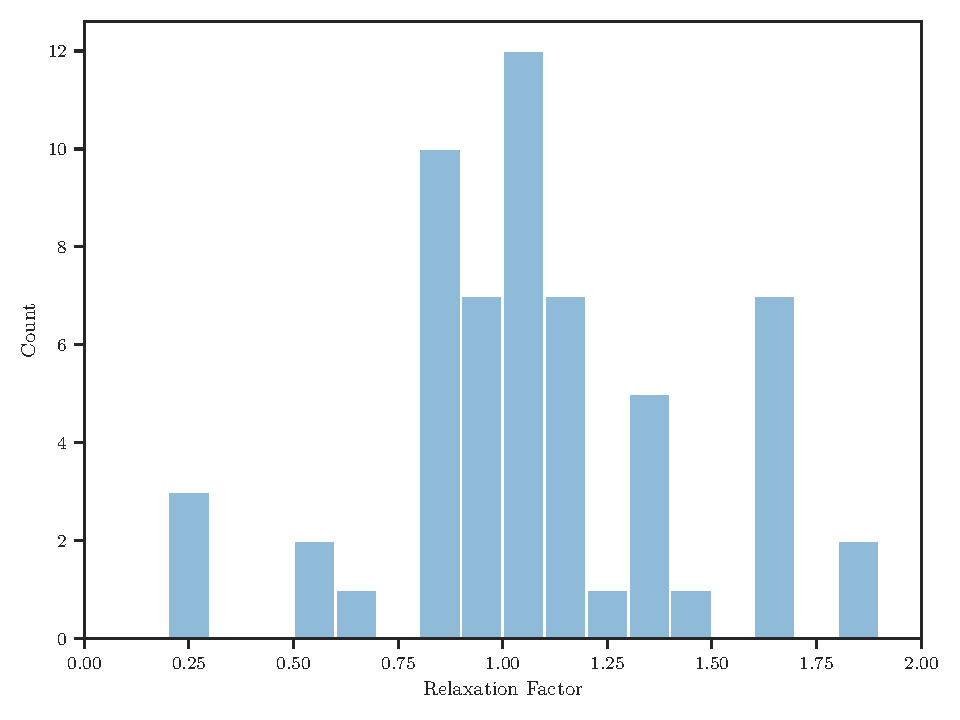
\includegraphics[height=0.4\textheight]{figures/histogram_cgc.pdf}
	\caption{Coarse-grid correction}
	\label{fig:histogram-rbgs}
\end{subfigure}
    \caption{Histogram of the relaxation factor distributions of the six multigrid-based preconditioners that yield a converging solver for $k = 640$.}
    \label{fig:histograms}
\end{figure} 